\section{Evaluation}
\label{sec.scheduling.evaluation}


\subsection{Methodology}
\begin{figure}[t]
	\centering
	\subfloat[Cholesky 8$\times$8]{
		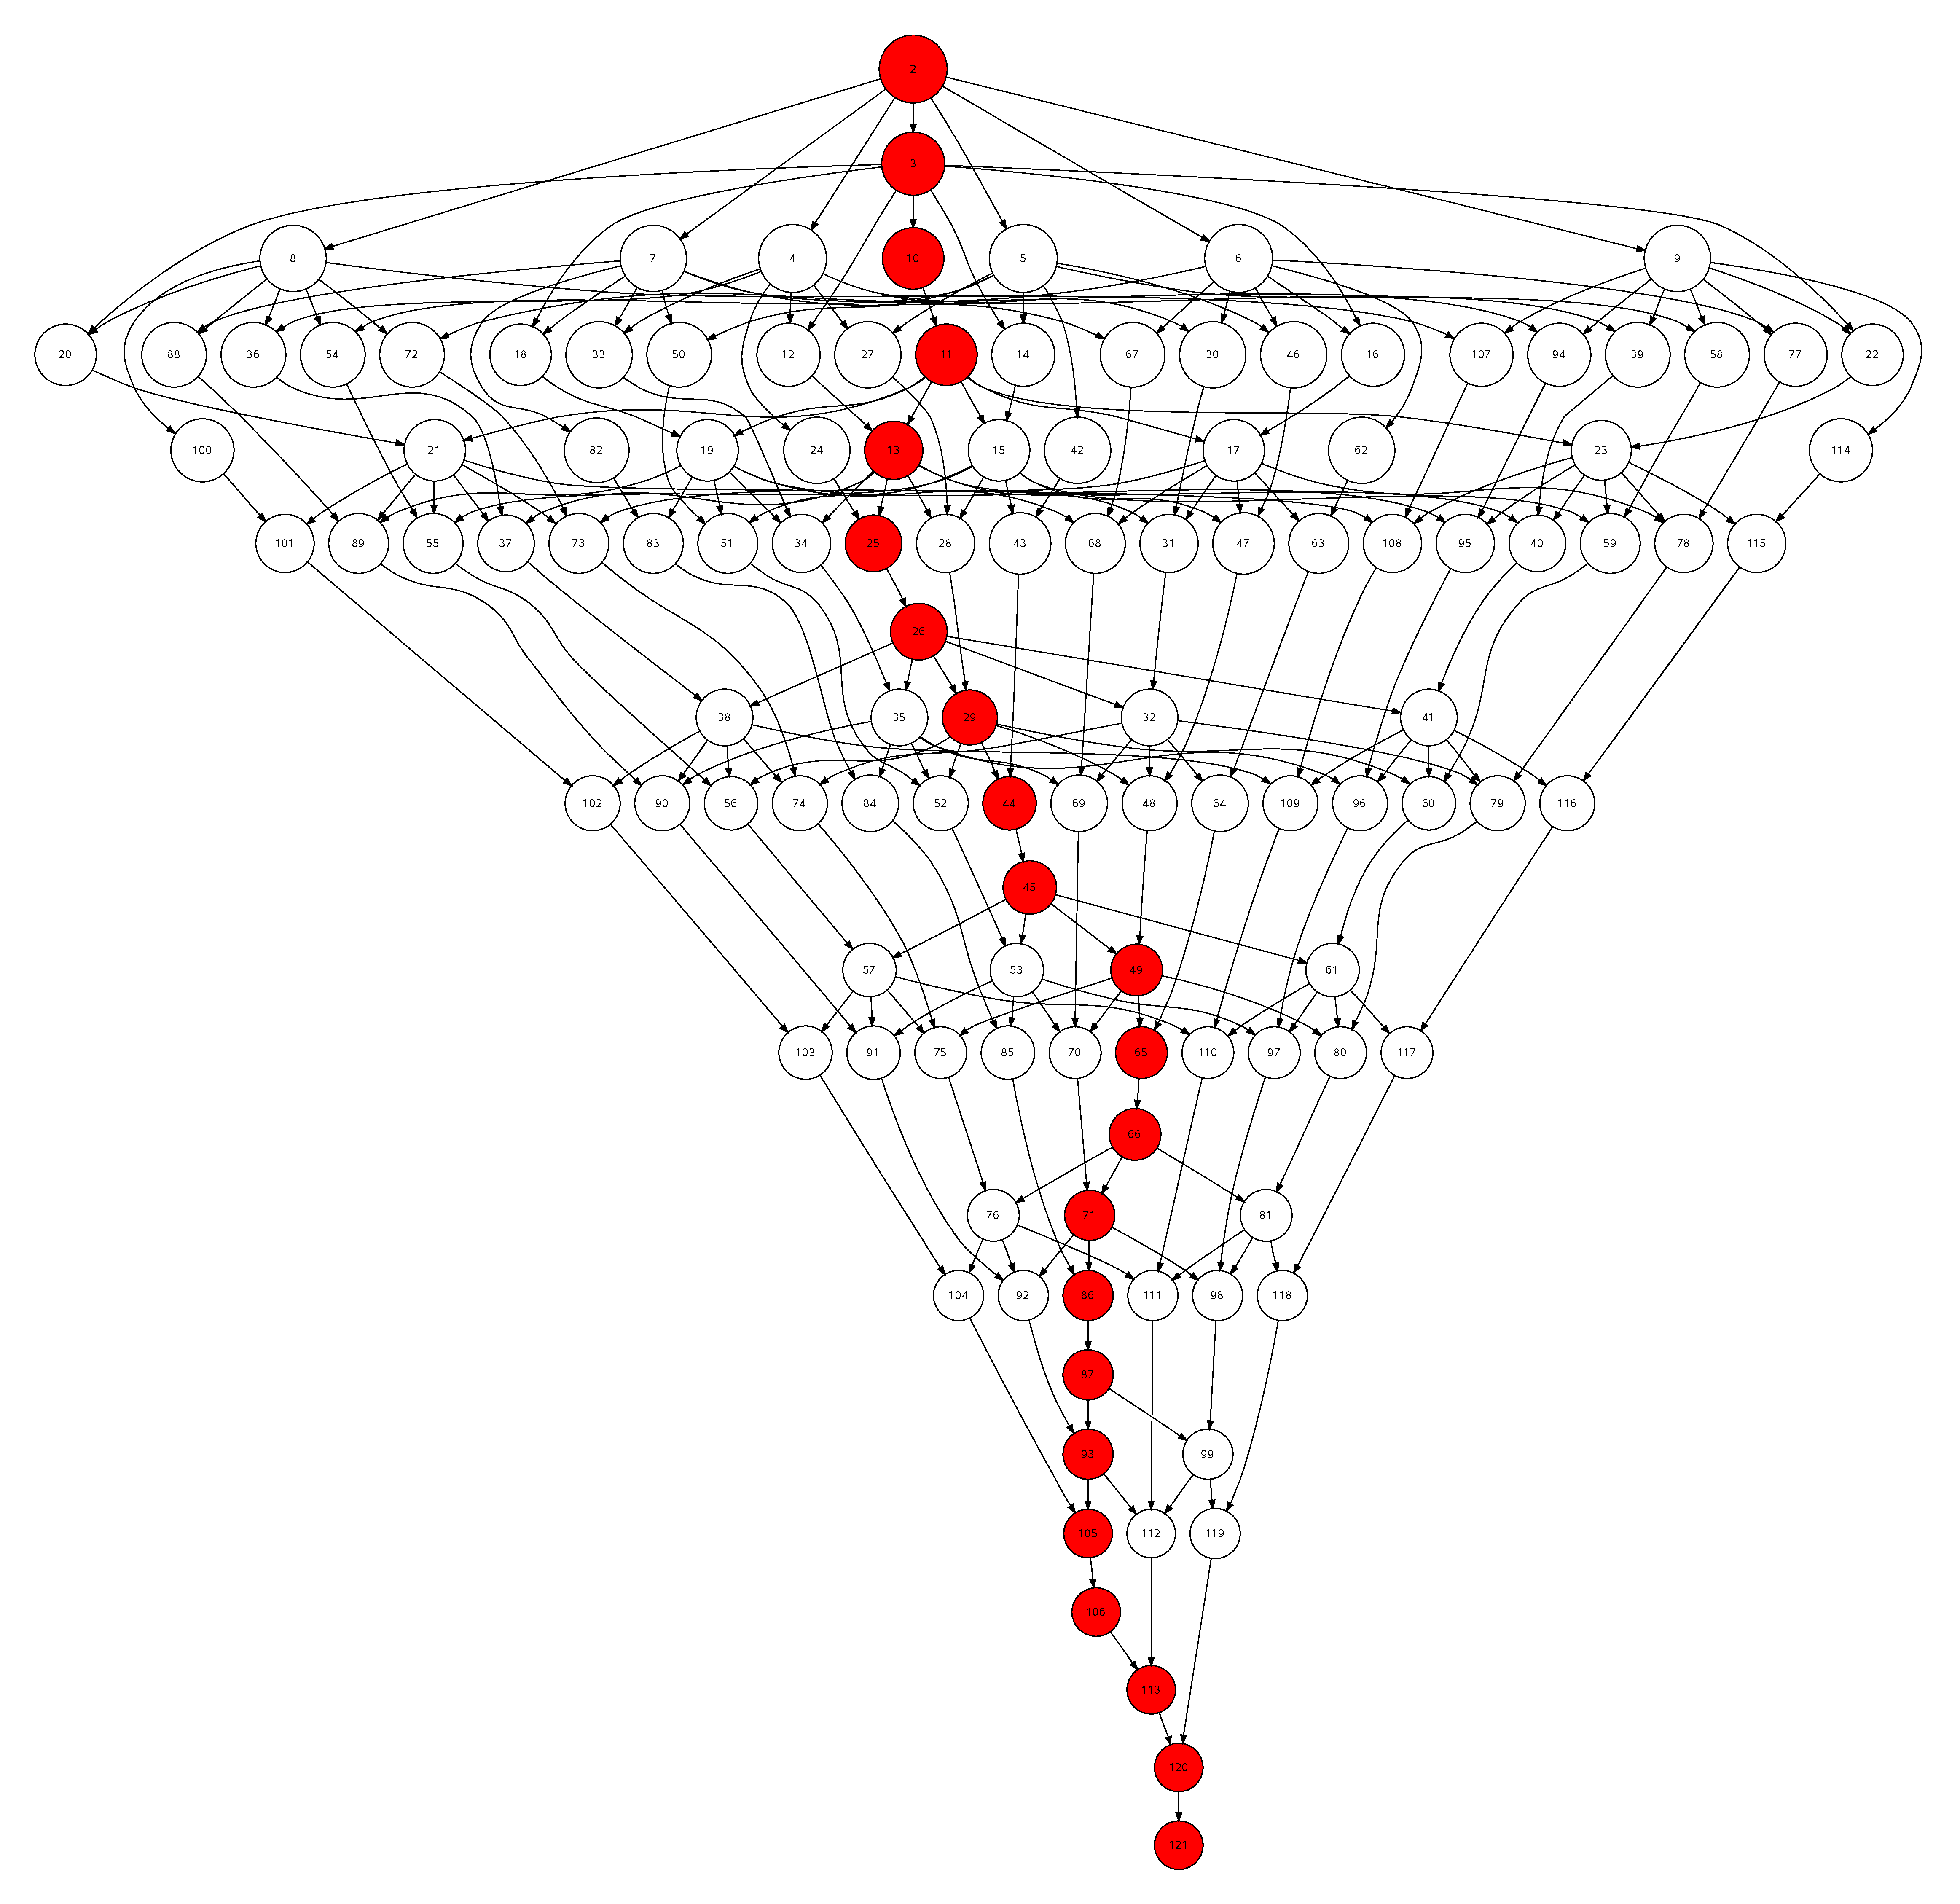
\includegraphics[width=0.26\textwidth]{images/cholesky_8_white.pdf}
		\label{cholesky8x8_TDG}
	}
	\subfloat[Cholesky 16$\times$16]{
		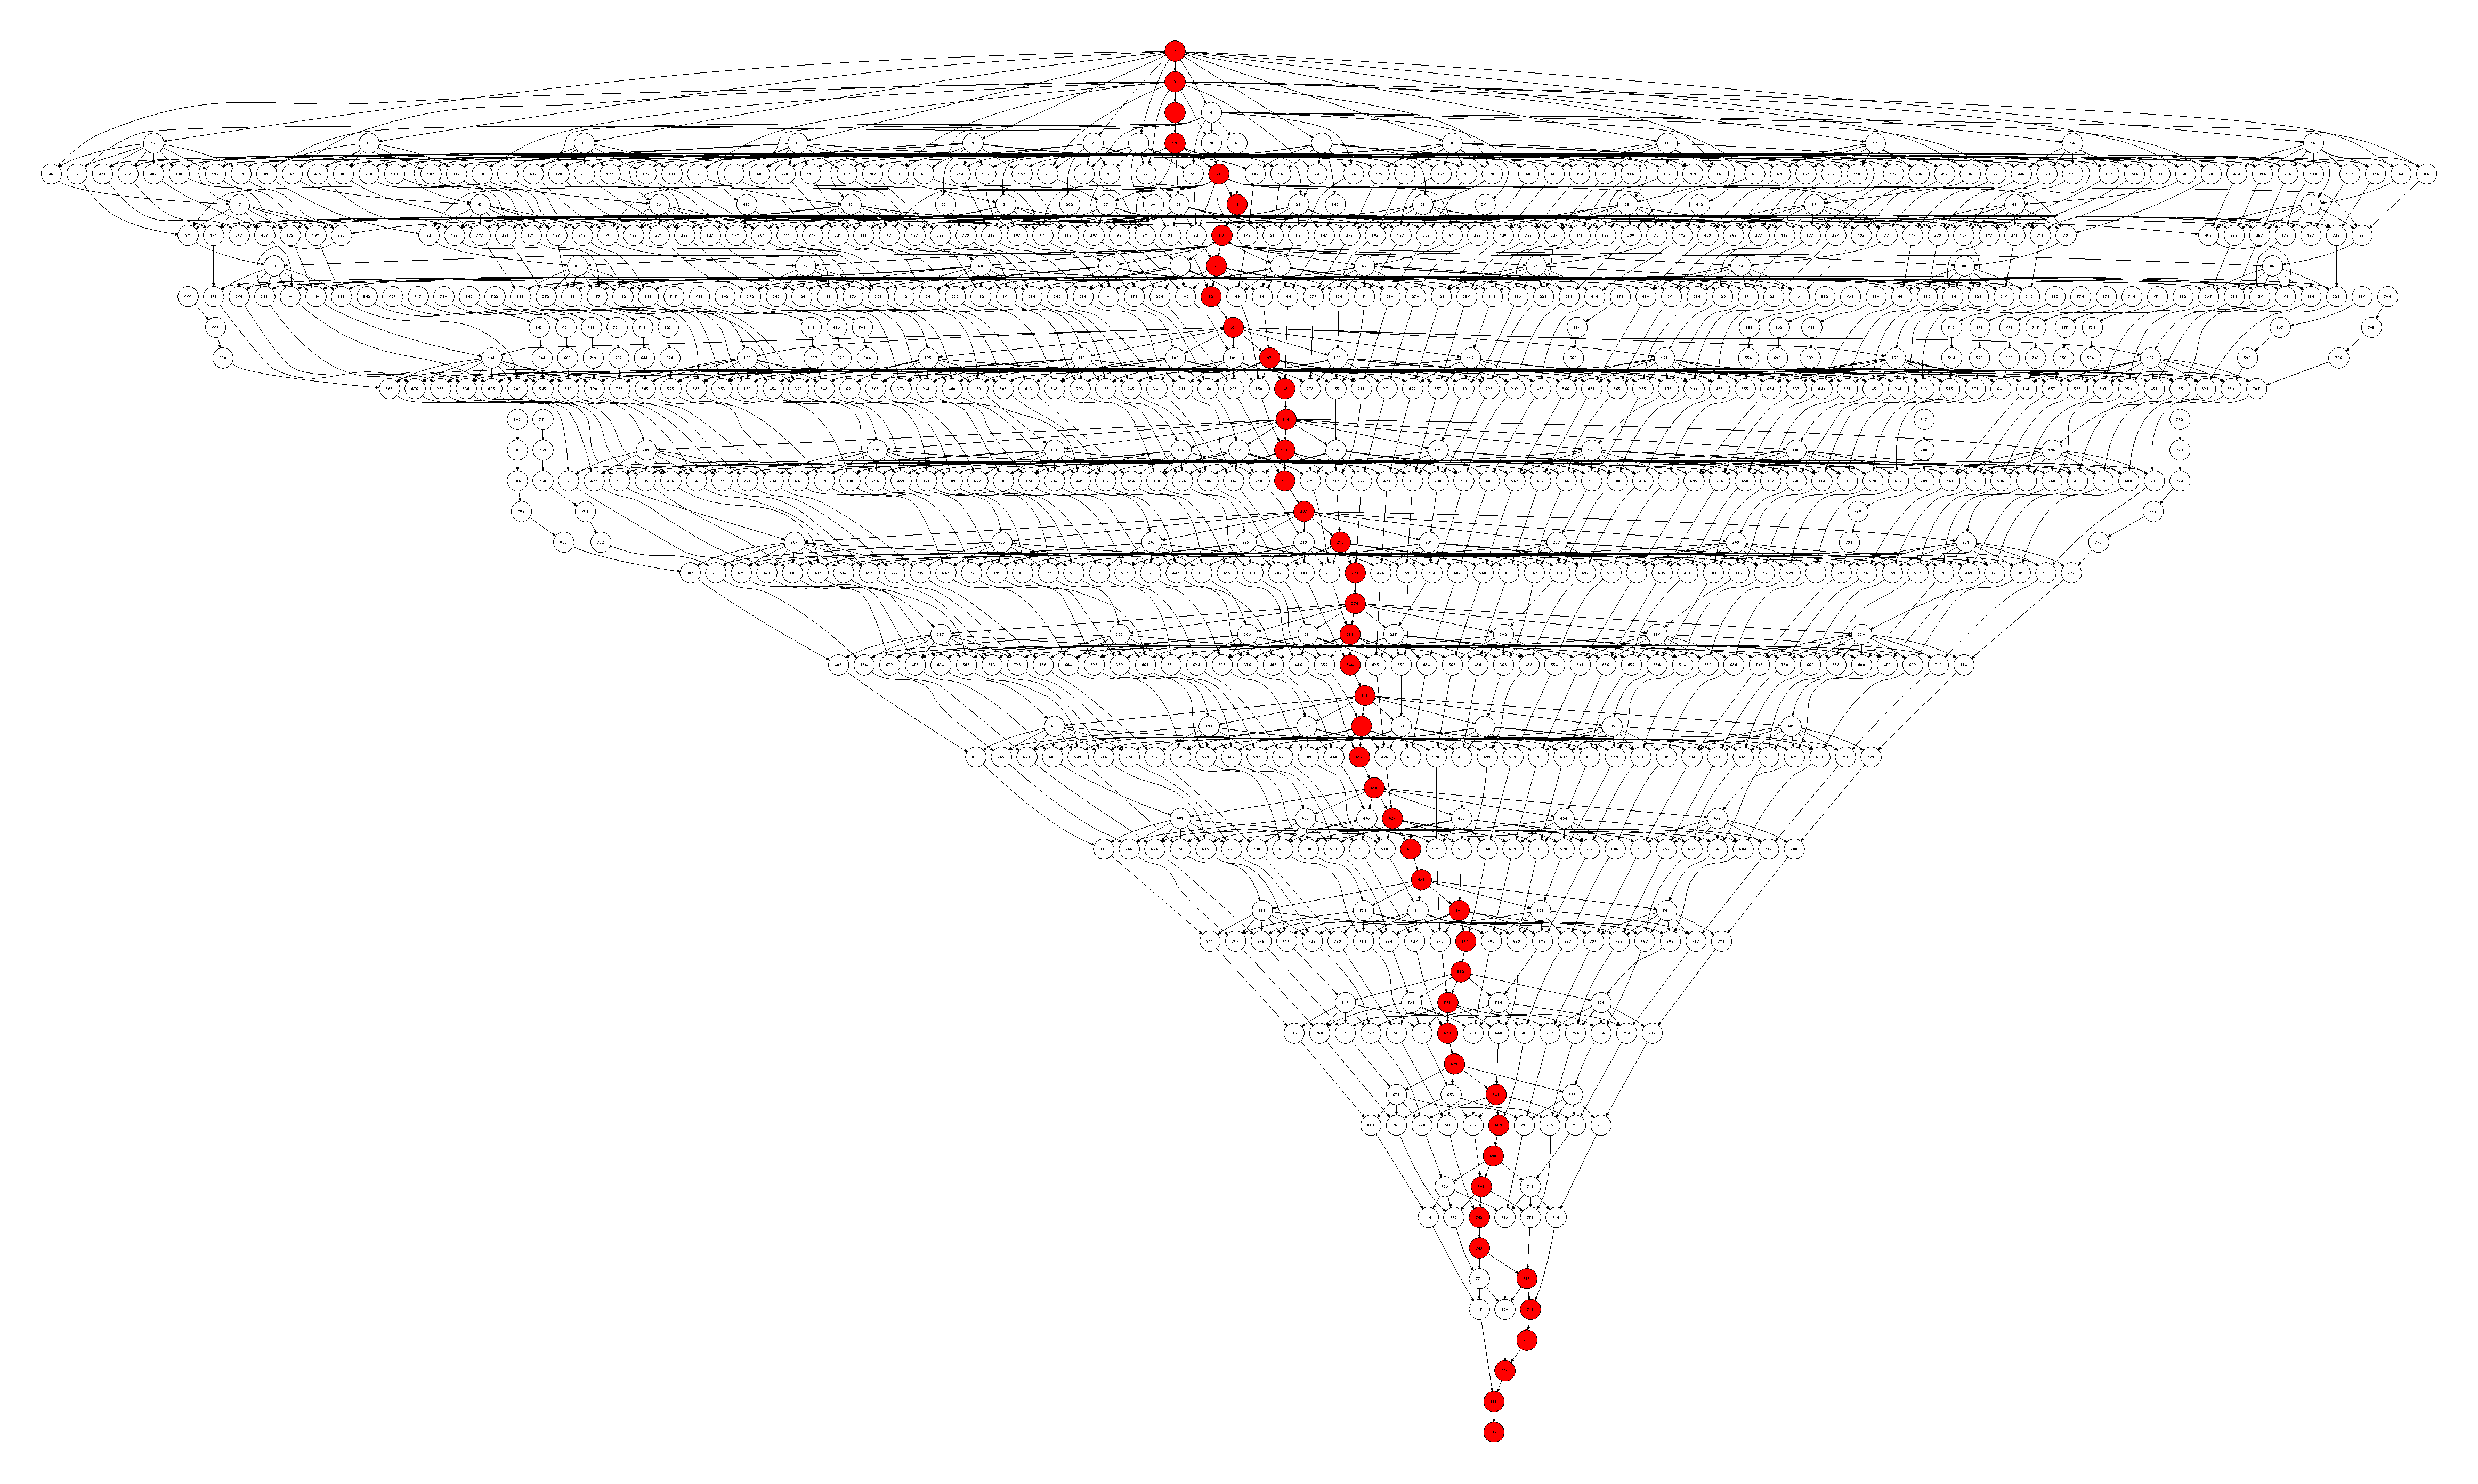
\includegraphics[width=0.6\textwidth]{images/cholesky_16_white.pdf}	
		\label{cholesky16x16_TDG}
	}
	\caption{Cholesky factorization task dependency graphs.}
	\label{fig.cholesky_graphs}
\end{figure}
% For example, a multi-core chip with some in-order cores and some out-of-order cores. The evaluation part of this paper contains real machine evaluation as well as evaluation through simulation.

%CATS targets heterogeneous multi-core systems with cores that expose different characteristics in terms of performance and power. We perform experiments on ODROID XU3 8-core platform. The ODROID XU3, features the ARM big.LITTLE technology offering heterogeneous multi-processing. Moreover, we simulate the behaviour of our design to estimate the impact of CATS on heterogeneous systems with a larger amount of cores and different performance ratios.
%On the simulated platform we are able to set up different performance ratios between fast and slow cores without a restriction.

In the first part of our real environment evaluation, we measure the execution time of four criticality-sensitive applications using CATS ad the default OmpSs scheduler. 
We evaluate four different CATS configurations based on the options explained in Section~\ref{sec.scheduling.cats} and provide a detailed comparison between them. 
The options consist of whether the task submission policy is strict or flexible, and the type of the work stealing mechanism. 
This results in the following configurations:
\begin{itemize}
	\itemsep0em
	\item Flexible with simple work stealing (SS FLEX)
	\item Flexible with bidirectional work stealing (2DS FLEX)
	\item Strict with simple work stealing (SS STRICT)
	\item Strict with bidirectional work stealing (2DS STRICT)
\end{itemize}

%\kc{should it stay or should it go???:}
As mentioned in Section~\ref{sec.background.taskbased.ompss}, the default OmpSs scheduler employs a \textit{breadth-first} policy~(BF)~\cite{Duran_schedulers_08}. 
The BF scheduler implements a single first-in-first-out ready queue shared among all threads. 
When a task is ready, it is inserted in the tail of the ready queue and when a core becomes available, it retrieves a task from the head of the queue. Tasks are ordered according to their ready time: the earliest ready task resides at the head of the queue. Since the ready queue is shared, there is no need for work stealing and the load is balanced automatically. BF does not differentiate among core types and assigns tasks in a first-come-first-served basis.

After the analysis of the CATS configurations we measure the execution time of five applications using CATS, CPATH, HYBRID, dHEFT and the default OmpSs BF scheduler that is explained in Section~\ref{sec.background.taskbased.ompss}. 
The execution time corresponds to the average of 10 executions of the application on each machine set-up.

%%%%%%%%%%%%%%%%%%%%%%%%%%%%%%%%%%%
\if 0 % about strict/flexible
As it is already shown in previous works~\cite{Chronaki:ICS2015}, the most efficient CATS configuration is when using the simple work stealing and flexible policy (SSFLEX).
The same applies for CPATH and HYBRID schedulers, thus the results presented in this section refer to this configuration of the schedulers. 
\fi %%%%%%%%%%%%%%%%%%%%%%%%%%%%%%%%
Our test bed comprises a real big.LITTLE processor and a simulated heterogeneous system.

%The default OmpSs scheduler employs a \textit{breadth-first} policy~(BF)~\cite{Duran_schedulers_08}. The BF scheduler implements a single first-in-first-out ready queue shared among all threads. When a task is ready, it is inserted in the tail of the ready queue and when a core becomes available, it retrieves a task from the head of the queue. Tasks are ordered according to their ready time: the earliest ready task resides at the head of the queue. Since the ready queue is shared, there is no need for work stealing and the load is balanced automatically. BF does not differentiate among core types and assigns tasks in a first-come-first-served basis. We use this scheduler as a baseline for the evaluation.

%%TODO this needs to be rephrased and more structured...
%We implement a dynamic version of HEFT scheduler (dHEFT) in the OmpSs programming model. The implementation assumes two different types of cores (big and little) and keeps records of the tasks' execution times in each core. The original HEFT \cite{HEFT} implementation assumes the prior knowledge of the TDG as well as the costs of the tasks. In our case, since the evaluation consists of running benchmarks, best way to compare HEFT and the other approaches is to keep the scheduling idea of HEFT and transform it from a static scheduler to a dynamic scheduler. This means that during runtime dHEFT discovers the costs of the tasks, computes a mean value of the costs for each task-type, parameter-size duple for each type of processor and then finds the processor that will finish the task at the earliest possible time. A difference between the static HEFT and dHEFT is the order that the tasks are being submitted. In HEFT tasks are submitted in decreasing order of their upward rank, which is computed statically with the known task costs. Since dHEFT discovers the costs while tasks are executing, there is no priority in the task submission. In dHEFT tasks are submitted as soon as they become ready. To find the earliest possible executor, dHEFT maintains one list per core (\textit{wlist}) with the ready tasks that are waiting to be executed by this core. When a task is submitted, dHEFT first checks if there are records of prior execution of this task. If the number of records is sufficient (in our experiments we use 3 records at least) then the estimated execution time of the task is considered stable. So, the task is scheduled to the earliest executor by consulting the \textit{wlist} of all the processors. If the number of records is not sufficient for one of the processor types then the task is scheduled to the earliest executor of this processor type. In any case dHEFT creates history by storing every time the task cost in the appropriate records in order to maintain stable results in the next submissions.

To perform our experiments, we use the Hardkernel \textbf{Odroid-XU3} development board that has an 8-core Samsung Exynos 5422 with an ARM big.LITTLE architecture. 
This platform is described in detail in section~\ref{sec.background.arm}.
%The Hardkernel \textbf{Odroid-XU3} development board has an 8-core Samsung Exynos 5422 chip with an ARM big.LITTLE architecture and 2GB of LPDDR3 RAM at 933MHz. The chip has four Cortex-A15 cores clocked at 1.6GHz and four Cortex-A7 cores at 800MHz. The four Cortex-A15 cores form a \textit{cluster} with a shared 2MB L2 cache, and the Cortex-A7 share a 512KB L2 cache. The two \textit{clusters} are coherent, so a single shared memory application can run on both clusters, using up to eight cores simultaneously. 
In our experiments, we evaluate a set of possible combinations of fast and slow cores varying the total number of cores from two to eight. 
%For the remainder of this section, we refer to Cortex-A15 cores as \textit{big} and to Cortex-A7 cores as \textit{little}.

% Talking about the performance ratio of the applications before describing the applications sound a bit strange, let's move this to applications section
%Depending on the workload, big and little cores expose different performance ratios. For example, a double precision benchmark advances a big core to be 3$\times$ faster than a little core, while for integer operations a big core is 1.9$\times$ faster than a little one \cite{Greenhalgh2011}. To get the notion of this performance ratio, we perform an execution of each application in one big core and another identical execution in one little core. The difference in performance on these two execution defines the difference in performance for big and little cores for each specific workload. Table \ref{tab.apps} shows the performance ratios explored for the benchmarks that we use.

%According to the calculated performance ratio, we can export the upper bound on speedup over a little core for each benchmark when running on 8 cores. Equation \ref{eq.ideal} shows how the ideal speedup is computed and assumes that the workload can be fully parallelized with zero dependencies, overheads or sequential sections in the application, according to Amdahl's law \cite{Amdahl}.
%\begingroup\makeatletter\def\f@size{9}\check@mathfonts
%\begin{equation}
%  \text{IDspeedup(workload, 8) = 4 $\times$ perf\_ratio(workload) + 4}
%\label{eq.ideal}
%\end{equation}
%\endgroup


%% Replaced for anonimity
%\subsubsection{TaskSim}

%Heterogeneous platforms such as ODROID-XU3 are currently limited in terms of size. We expect that future heterogeneous platforms will grow bigger with a larger amount of cores and various performance differences between fast and slow cores. 
To evaluate heterogeneous scheduling on larger multi-core systems we use the heterogeneous multi-core TaskSim simulator~\cite{AbstrLevels_TACO12} described in section~\ref{sec.background.simulation}. TaskSim allows the specification of a heterogeneous system with two different types of cores: fast and slow. 
We can configure the amount of cores of each type and the difference in performance between the different types (performance ratio) in the TaskSim configuration file.
In our experiments, we evaluate the effectiveness of the schedulers on 8 distinct heterogeneous machine configurations. 
These comprise systems with 16 or 32 total number of cores, and the number of fast cores ranging from 1 to 16. 
We set the performance ratio between fast and slow cores to 4.5$\times$ because this is the average performance ratio observed on the real machine for the benchmarks of this evaluation.

%For all these configurations, we evaluate the following performance ratios between fast and slow cores: 2$\times$, 2.5$\times$, 3$\times$, 3.5$\times$ and 4$\times$.

%% moved here because we needed to know about the heterogeneous platforms before talking about big and little cores

%The metric used in the following charts for each pair (\textit{total number of cores, number of big cores}), is the improvement of CATS over the baseline scheduler as well as the speedup obtained for each policy over one LITTLE core. The improvement is computed as shown in Equation~\ref{eq.improvement} and the speedup is computed as shown in Equation~\ref{eq.speedup}.

%% This, we are already saying in the explanation of the platforms
%

For both real and simulated platforms, each set-up has a given number of \textit{total} and \textit{big} cores.
%Our metrics are the improvement of CATS over the baseline scheduler, and the 
For all the scheduling approaches we present their speedup over the execution on one \textit{little} core, shown in Equation~\ref{eq.sched.speedup}. 
%Equations~\ref{eq.improvement} and~\ref{eq.speedup} show the improvement and speedup calculations.
%Equation~\ref{eq.speedup} shows how speedup is calculated in this evaluation.
\begingroup\makeatletter\def\f@size{8}\check@mathfonts
%\begin{equation}
%  \text{Improv. over BF(total, big)} = \frac{\text{Exec. time BF(total, big)}}%{\text{Exec. time CATS(total, big)}}
%\label{eq.improvement}
%\end{equation}
\begin{equation}
  \text{Speedup(total, big)} = \frac{\text{Exec. time(1, 0)}}{\text{Exec. time(total, big)}}
  \label{eq.sched.speedup}
\end{equation}
\endgroup


\subsubsection{Applications}

\begin{table*}
	\scriptsize
	\begin{center}
		\caption{Evaluated benchmarks and relevant characteristics. The inputs of QR and Heat diffusion are arrays of doubles and the inputs of Cholesky and Int. Histogram are arrays of floats.}
		\label{tab.sched.apps}
		\begin{tabular}{|c|c|c|c|c|c|c|c|c|}
			\hline
			\multirow{2}{*}{\parbox{10mm}{\centering Application}} & 
			\multirow{2}{*}{\parbox{9mm}{\centering Problem size}} & 
			\multirow{2}{*}{\parbox{9mm}{\centering \#Tasks}} & 
			\multirow{2}{*}{\parbox{9mm}{\centering \#Task types}} & 
			\multirow{2}{*}{\parbox{18mm}{\centering Avg task exec. time (${\mu}s$)}} & 
			\multicolumn{3}{|c|}{Per task overheads (${\mu}s$)} &\\
			\cline{6-8}
			& & & & & {\parbox{10mm}{\centering CATS}} & {\parbox{10mm}{\centering CPATH}} & {\parbox{11mm}{\centering HYBRID}} &
			
			\multirow{2}{*}{\parbox{13mm}{\centering Measured perf. ratio}} \\
			& & & & & & & & \\ %\hhline{~~~~~~}
			\hline
			
			\multirow{3}{*}{Cholesky} 
			& 8K 1024 & 120 & & 10\,314\,660 & 81.19 &  115.29 &  112.41 & \\                                              
			& 8K 512 & 816 & 4 & 1\,551\,322 & 104.76 &  238.02 &  194.28 &3.48 \\ 
			& 16K 512 & 5984 & & 1\,551\,322 & 104.76 &  238.02 &  194.28  & \\ 
			\hline{}
			QR & 8K 512 & 1\,496 & 4 & 11\,651\,079  &   1\,419.33 & 2\,580.41 &   1\,451.74 & 6.86 \\ 
			\hline
			Heat diffusion & 8K 512 & 5\,124 & 3 & 93\,198  &   145.17  &  748.84 &  170.00& 3.68 \\
			\hline
			Int. Histogram & 8K 512 & 2\,048 & 2 & 514\,096 &  217.45 &  62.07 & 263.62  & 2.23 \\ 
			%Heat diffusion & Heat &  &  &  &  &  & \\ 
			\hline
			Bodytrack & native & 408\,525 &  6 & 41\,869 & 93.90 & 120.93 &  120.93 & 4.14 \\
			\hline
		\end{tabular} 
	\end{center}
\end{table*}
\normalsize
\begin{figure}[t]
	\centering
	\subfloat[Cholesky 8$\times$8]{
		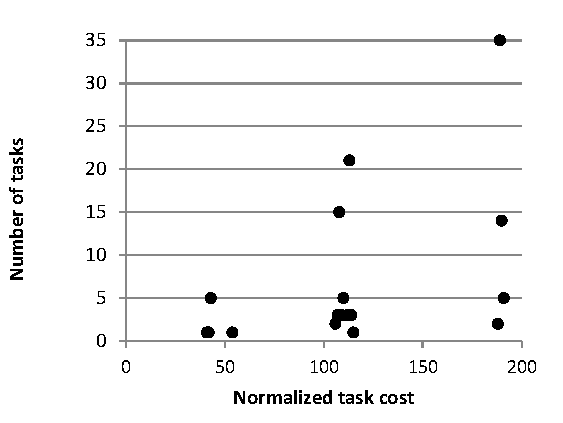
\includegraphics[width=0.3\textwidth]{images/cholesky_8x8_distribution.pdf}
		\label{cholesky8x8_dist}
	}
	\subfloat[Cholesky 16$\times$16]{
		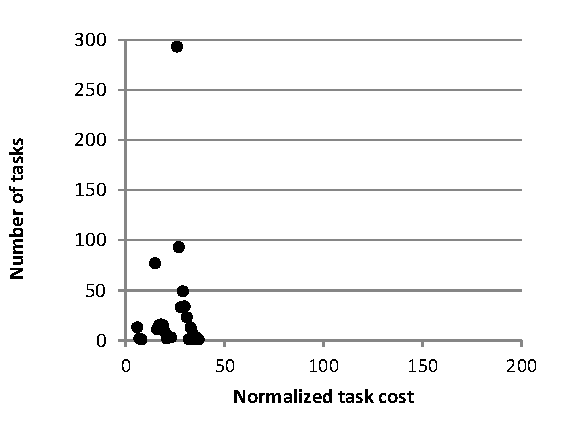
\includegraphics[width=0.3\textwidth]{images/cholesky_16x16_distribution.pdf}	
		\label{cholesky16x16_dist}
	}
	\subfloat[QR factorization]{
		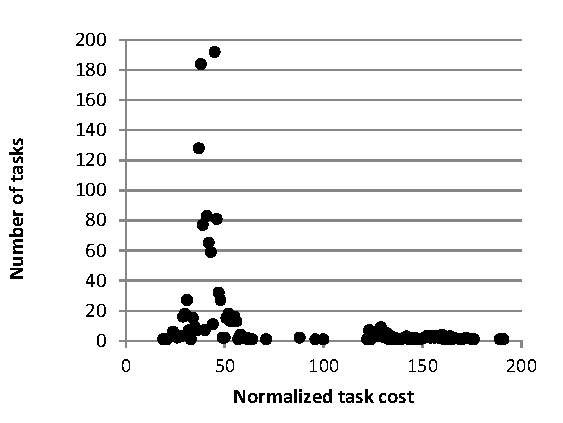
\includegraphics[width=0.3\textwidth]{images/QR_16x16_distribution.pdf}	
		\label{qr_dist}
	}
	\\
	\subfloat[Heat diffusion]{
		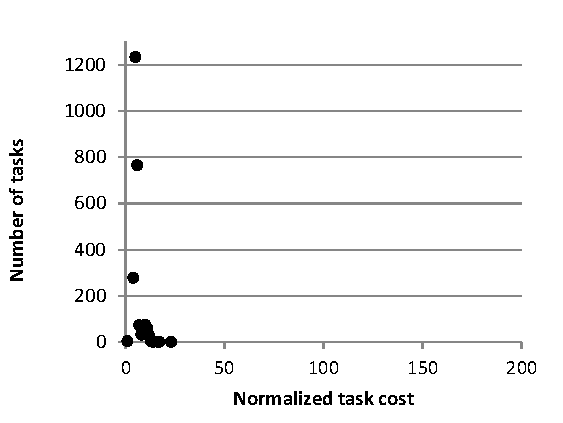
\includegraphics[width=0.3\textwidth]{images/heat_16x16_distribution.pdf}	
		\label{heat_dist}
	}
	\subfloat[Integral Histogram]{
		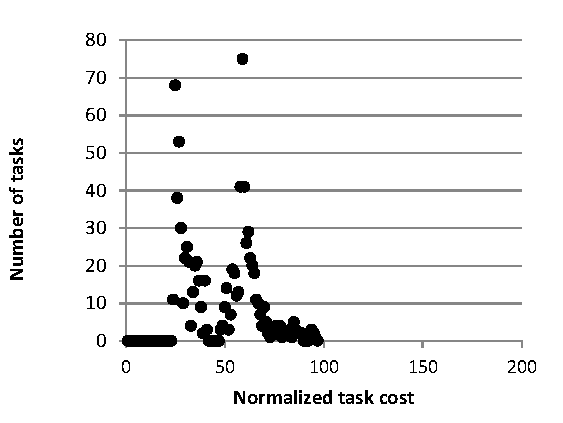
\includegraphics[width=0.3\textwidth]{images/histogram_8x8_distribution.pdf}	
		\label{histogram_dist}
	}
	\subfloat[Bodytrack]{
		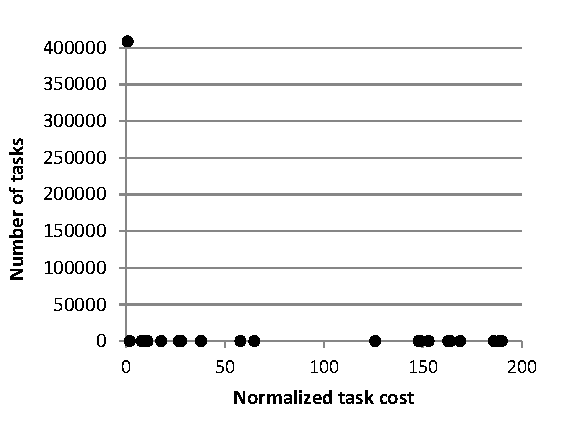
\includegraphics[width=0.3\textwidth]{images/bodytrack_native_distribution.pdf}	
		\label{bodytrack_dist}
	}
    \caption{Task cost distribution for each application. Results are based on 4BIG-core executions. $x$ axis shows the cost of the tasks and $y$ axis shows the number of tasks with the corresponding task cost.}
  \label{distributions}
  %\vspace{-0.4cm}
\end{figure}

We use five scientific applications implemented in the OmpSs programming model: Cholesky factorization, QR factorization, Heat diffusion, Integral Histogram and Bodytrack, also described in Section~\ref{sec.background}. 
These benchmarks are accessible in the BSC Application Repository~\cite{BAR} and in the PARSECSs library~\cite{Chasapis:TACO2016}. 


%\subsubsection{Bodytrack}
%\textbf{Bodytrack} is an application that tracks a marker-less human body using multiple cameras through an image sequence. 
%The OmpSs version implements a two-stage parallel pipeline for the image processing.
%%In the first stage the implementation allows the concurrent processing of all the frames of the image sequence. 
%%The second stage is the application of a particle filter to the images in order to mark the human body.
%The two stages are synchronized through the OmpSs dataflow annotations.
%By allowing the parallel processing of frames, OmpSs achieves the overlapping of the I/O and serial code with the tasks. 
%We use the native input of the benchmark suite~\cite{Chasapis:TACO2016}.

%Their different configurations and characteristics are shown in Table~\ref{tab.apps}.
%
%The applications have different sensitiveness depending on the inter-task dependencies that determine the available parallelism and the percentage of critical tasks, shown in the table. The larger proportion of critical tasks, the larger the potential improvement of CATS, as these are tasks that, once accelerated, reduce the application overall execution time. The percentage of critical tasks in Table~\ref{tab.apps} is from a single-core execution of CATS. Since CATS is dynamic, the tasks considered critical would be different for different configurations, since the algorithm runs on a partial dependency graph, including only the outstanding tasks. However, the single-core figures serve as an estimation of the percentage of critical tasks intrinsic to the overall application, that allows us to reason about the results with respect to this application characteristic.
%
%The percentage of critical tasks characterises the shape of the task dependency graph. The larger the proportion of critical tasks, the narrower the graph. These percentages, are exported from a single-core CATS execution of each kernel. So, this shows the theoretical amount of critical tasks that CATS discovers, since a multi-core execution of the application would detect the longest path dynamically. Nevertheless, it is shown experimentally that an application with a higher theoretical percentage of critical tasks has a higher number of critical tasks in practice, than an application with a small theoretical percentage of critical tasks.
%
%Depending on the workload, big and little cores expose different performance ratios. For example, a double precision benchmark advances a big core to be 3$\times$ faster than a little core, while for integer operations a big core is 1.9$\times$ faster than a little one \cite{Greenhalgh2011}. To get the notion of this performance ratio, we perform an execution of each application in one big core and another identical execution in one little core. The difference in performance on these two execution defines the difference in performance for big and little cores for each specific workload. Table \ref{tab.apps} shows the performance ratios explored for the benchmarks that we use.
%IDEAL SPEEDUP
%The performance ratios in Table~\ref{tab.apps} are computed for the real machine by comparing the execution time on one little core over the execution time on one big core. Using these performance ratios, we can estimate the ideal speedup over a little core for each application running on all eight cores. Equation~\ref{eq.ideal} is used for the ideal speedup. The ideal speedup considers a fully parallel workload, without any dependencies, overheads or sequential sections, thus unachievable by the dependency-intensive applications in our evaluation.%in the application, according to Amdahl's law \cite{Amdahl}.
%\begingroup\makeatletter\def\f@size{7}\check@mathfonts
%\begin{equation}
%  \text{ideal\_speedup(workload, 8) = 4 $\times$ perf\_ratio(workload) + 4}
%\label{eq.ideal}
%\end{equation}
%\endgroup
%END IDEAL SPEEDUP

Table \ref{tab.sched.apps} shows the different configurations and characteristics of the applications.
For cholesky, QR, heat diffusion and integral histogram the input is a square matrix divided into blocks.
The \textit{Problem size} column of Table~\ref{tab.sched.apps} shows the dimension of the input matrix and the block size.
For example cholesky 8K 1024 takes as input a matrix of 8192$\times$8192 and it is then divided to 8$\times$8 blocks of 1024 elements each.
Each task created in the parallelized versions operates on one block.
The bigger the block size, the less the number of blocks created, which leads to less tasks. 
From the applications of Table~\ref{tab.sched.apps}, QR and Heat diffusion operate on doubles while Cholesky and Integral Histogram operate on floats.
The performance ratio between big and little cores depends on the application. 
For example, the difference between the issue rate and throughput of double-precision floating point units of both types of cores is larger than the difference for single-precision floating point instructions. Therefore, applications with heavy double-precision operation (e.g. QR) get a larger benefit from running on the big cores, than single-precision dominated applications (e.g integral histogram), as shown in Table~\ref{tab.sched.apps}.

The average per task overhead for each scheduler is negligible compared to the average task execution time shown in Table~\ref{tab.sched.apps}. Specifically, CATS has the lowest per task overheads. Next is HYBRID and the least efficient is CPATH. This is because of the complexity of the CPATH algorithm that takes place whenever the TDG needs to be updated.
On the other hand, CATS and HYBRID have negligible overheads caused by the task prioritization.
For dHEFT, the search of the appropriate worker for a task becomes an obstacle in performance. 
Table~\ref{tab.sched.apps} lacks the per task overheads of dHEFT because they appear to be too high due to the fact that the most intensive computations of dHEFT take place during the cores' idle time.
Thus, the natural idle time of cores is also encountered as scheduling overhead and could not be separated, so it is unfair to present such results for comparison. 
Normally these obstacles in heterogeneous schedulers are paid off by the more effective task execution. 

Figure~\ref{fig.cholesky_graphs} shows the TDGs for input sizes of (a) 8$\times$8 and (b) 16$\times$16 blocks.
Critical tasks are denoted as red nodes. 
The TDG becomes wider as the number of blocks increases. 
This reduces the percentage of critical tasks that is 17.5\% in the case of the 8$\times$8 input and 5.51\% in the case of the 16$\times$16 input. 
The 8$\times$8 blocks case shows a narrower TDG that makes the application more criticality sensitive than the 16$\times$16 blocks case that exposes more parallelism. 
We evaluate both configurations to show the impact of scheduling on different criticality sensitiveness of the application configuration.

To more precisely characterise the benchmarks, we plot the task cost variability for each benchmark on Figure~\ref{distributions}.
We normalize the task execution time of the applications with respect to the smaller task observed among all applications so that we can easily compare the task sizes of different applications as shown on the distributions.
For each of these plots, the $x$ axis shows the normalized task cost (i.e. task execution time) and the $y$ axis the number of tasks that correspond to this task cost (e.g. how many tasks have this cost).
This is used in the next section to classify how heterogeneous each application is and explain the behavior of the heterogeneous schedulers that take into account the execution time.
%\subsubsection{Cholesky Factorization}



%\begin{figure*}[!t]
%	\centering
%	
%		\begin{subfigure}[b]{0.45\textwidth}
%		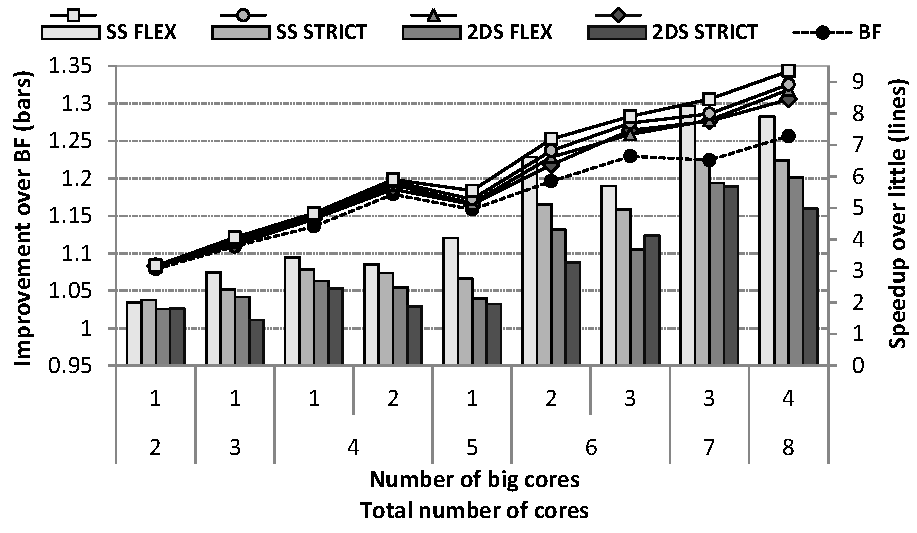
\includegraphics[width=\textwidth]{figures/cholesky_8x8_CATS.pdf}
%		\caption{Cholesky 8$\times$8}
%		\label{cholesky8x8_real}
%	\end{subfigure}
%	\begin{subfigure}[b]{0.45\textwidth}
%		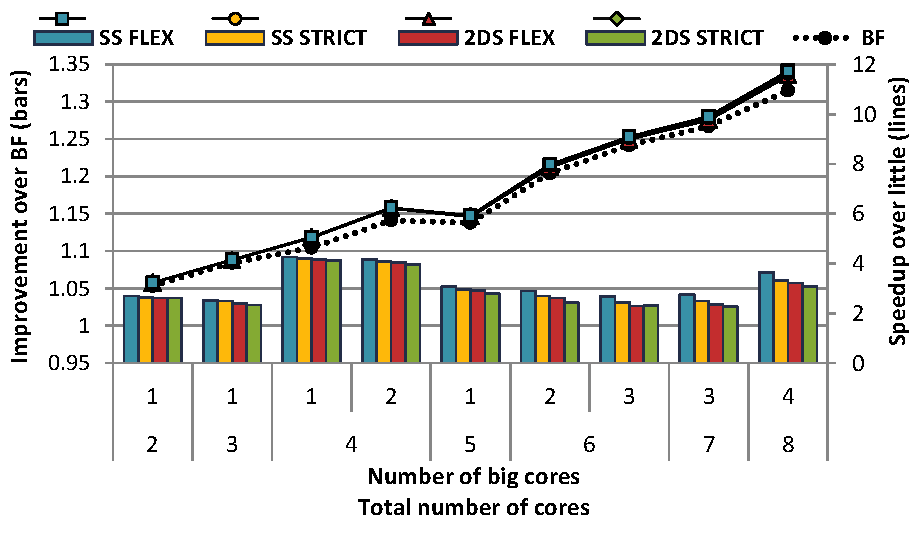
\includegraphics[width=\textwidth]{figures/cholesky_16x16_CATS.pdf}
%		\caption{Cholesky 16$\times$16}
%		\label{cholesky16x16_real}
%	\end{subfigure}
%	\begin{subfigure}[b]{0.45\textwidth}
%		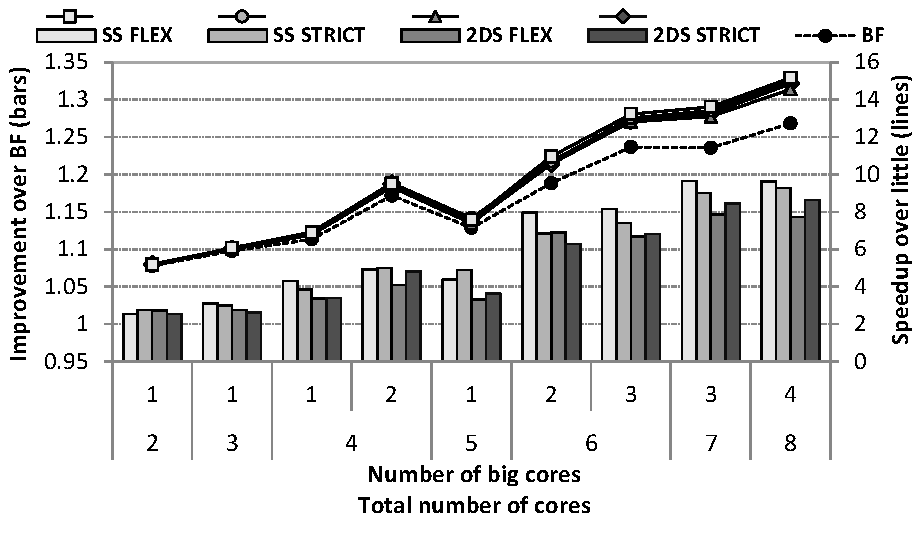
\includegraphics[width=\textwidth]{figures/QR_CATS.pdf}
%		\caption{QR}
%		\label{qr_real}
%	\end{subfigure}
%	\begin{subfigure}[b]{0.45\textwidth}
%		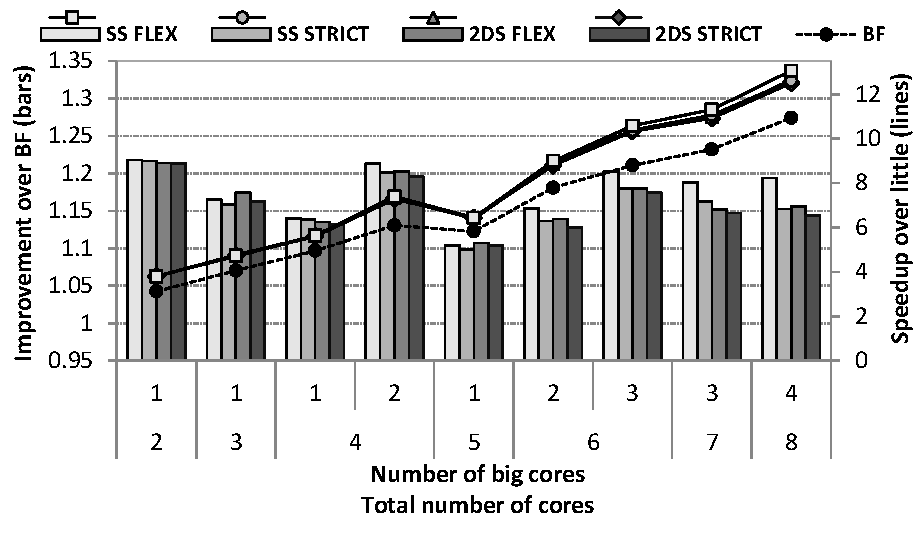
\includegraphics[width=\textwidth]{figures/heat_CATS.pdf}
%		\caption{Heat Diffusion}
%		\label{heat_ARM}
%	\end{subfigure}
%	\begin{subfigure}[b]{0.45\textwidth}
%		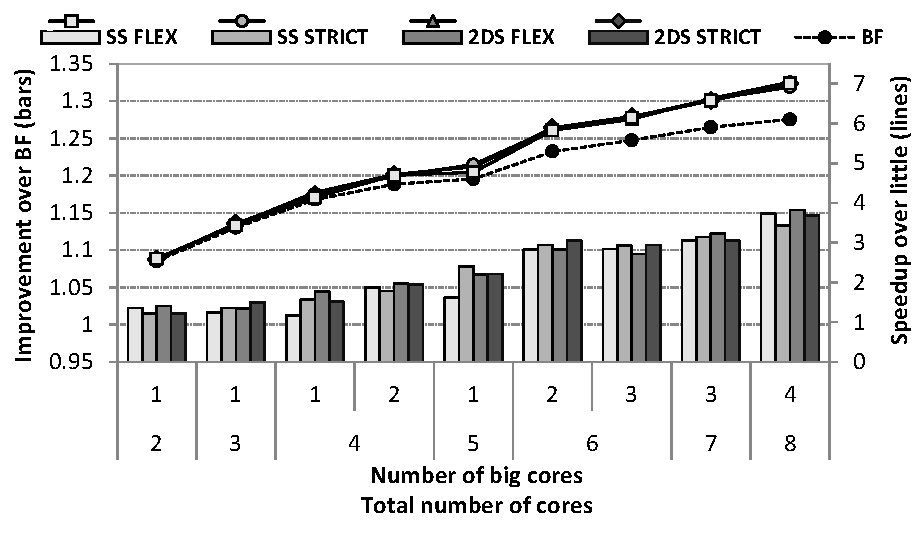
\includegraphics[width=\textwidth]{figures/intHist_CATS.pdf}
%		\caption{Integral Histogram}
%		\label{histogram_real16}
%	\end{subfigure}
%	\caption{Schedulers comparison on ODROID-XU3}
%	\label{eval_ARM}
%	\vspace{-0.4cm}
%\end{figure*}

\subsection{Real Environment Evaluation}
This subsection includes all the experiments and results obtained from the real asymmetric system ODROID-XU3.
It includes one section that explores the different CATS configurations and another section that compares the best CATS configuration among the rest of the schedulers.

\subsubsection{Evaluation of CATS Configurations}
\label{sec.cats_eval}
\begin{figure}[!t]
	\centering
		\subfloat[Speedup of CATS and BF compared to the ideal]{
		\includegraphics[width=0.45\textwidth]{figures/ideal_CATS.pdf}
		\label{BFlinear}
	}
	\subfloat[Cholesky 8$\times$8]{
		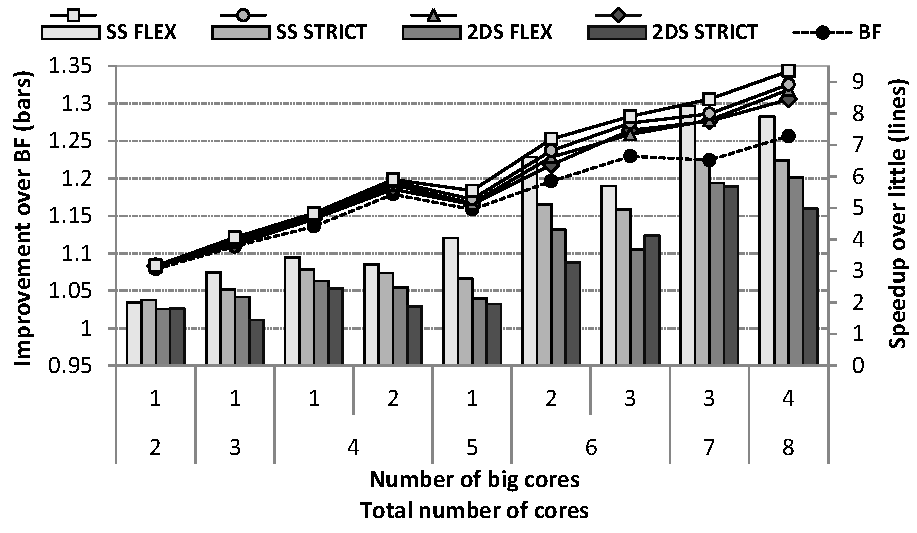
\includegraphics[width=0.45\textwidth]{figures/cholesky_8x8_CATS.pdf}
		\label{cholesky8x8_cats}
	}
	\\
	\subfloat[Cholesky 16$\times$16]{
		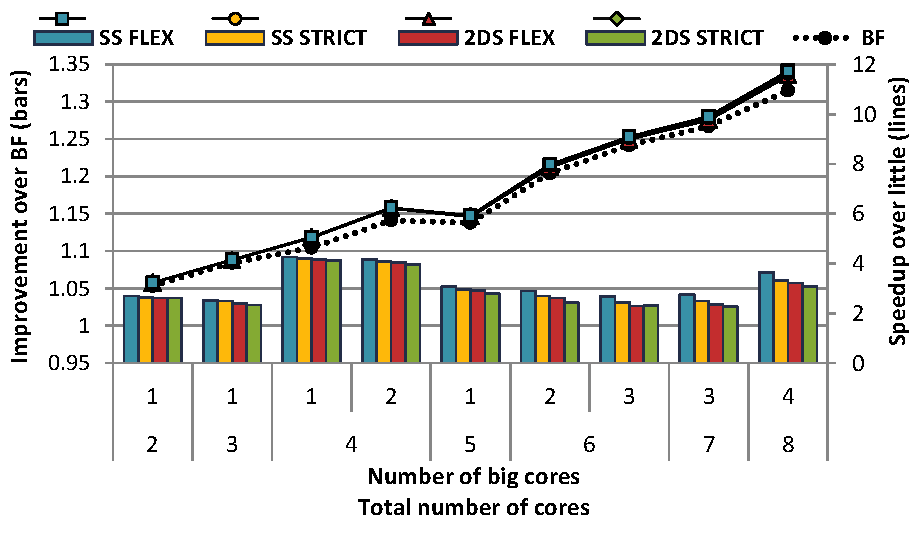
\includegraphics[width=0.45\textwidth]{figures/cholesky_16x16_CATS.pdf}
		\label{cholesky16x16_cats}
	}
	\subfloat[QR]{
		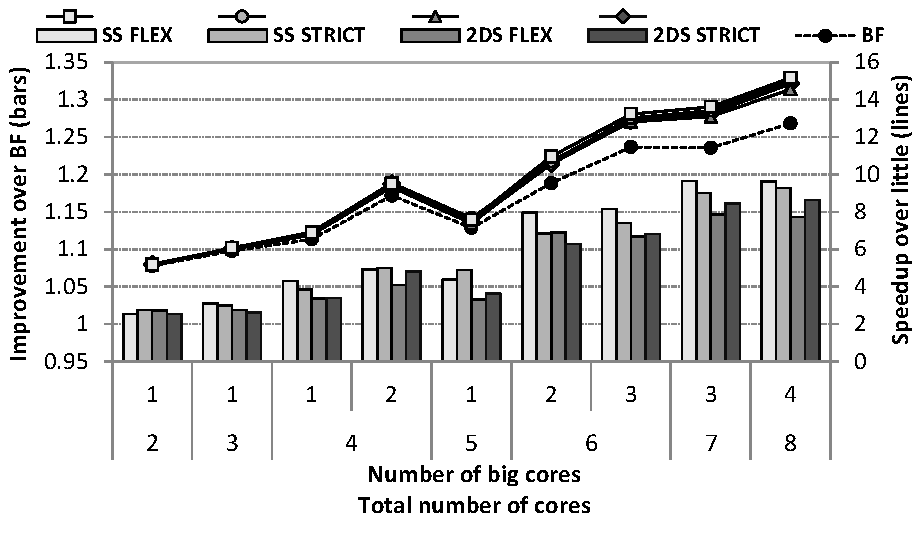
\includegraphics[width=0.45\textwidth]{figures/QR_CATS.pdf}
		\label{qr_cats}
	}
	\\
	\subfloat[Heat diffusion]{
		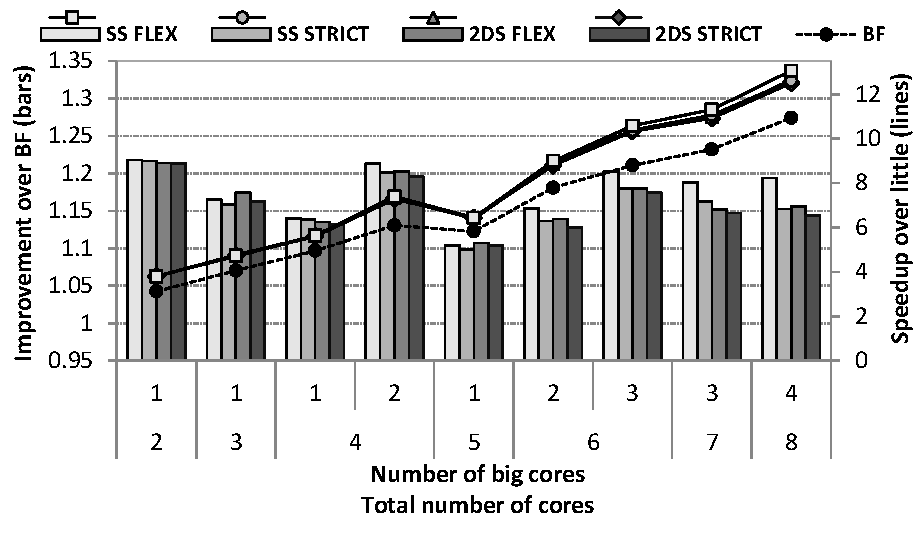
\includegraphics[width=0.45\textwidth]{figures/heat_CATS.pdf}
		\label{heat_cats}
	}
	\subfloat[Integral Histogram]{
		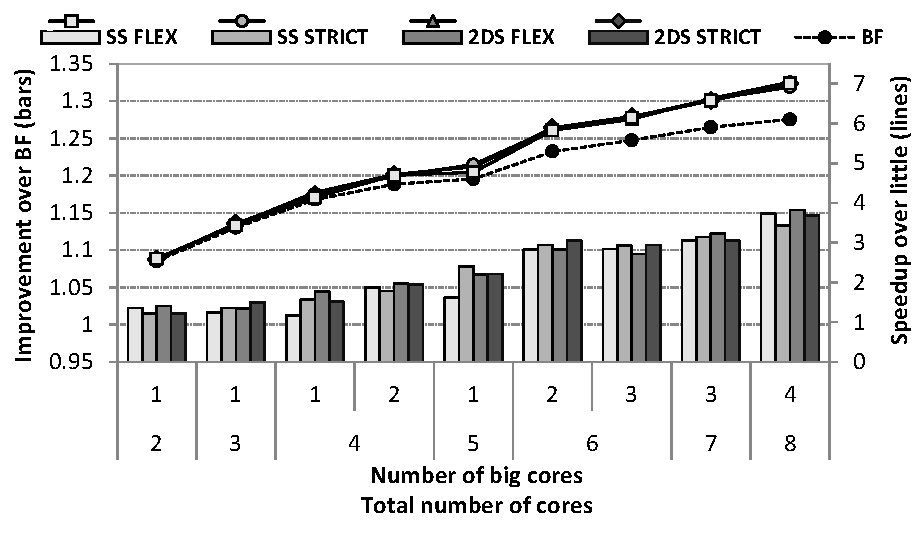
\includegraphics[width=0.45\textwidth]{figures/intHist_CATS.pdf}
		\label{histogram_cats}
	}
	%  \vspace{-0.2cm}
	\caption{Schedulers comparison on ODROID-XU3}
	%\vspace{-0.5cm}
\end{figure}
Figure~\ref{cholesky8x8_cats} shows the improvement of the CATS configurations over BF, and the speedup obtained with CATS and BF, for Cholesky on an 8$\times$8 blocked matrix. 
CATS consistently achieves better performance than BF and the improvement over BF increases as the number of cores is increased. 
Specifically, the improvement is observed to be up to 30\% for systems with seven and eight cores. 

Figure~\ref{cholesky16x16_cats} shows the performance on a 16$\times$16 block input matrix, where the improvement of CATS is smaller and ranges from 2 to 9\% and all schedulers perform fairly well. 
In this case the opportunities for enhancement are limited, since, according to Figure~\ref{BFLinear}, BF performance approaches the ideal speedup. 
The lower improvement in this case comes from the fact that the application is less sensitive to the critical path. 
The task graph is wider (as shown in Figure~\ref{fig.cholesky_graphs}) and, accordingly, the percentage of critical tasks is lower. 
Specifically the percentage of critical tasks for this input is limited to 5.5\% compared to the percentage observed with Cholesky 8$\times$8 that is 17.5\%. 
However, CATS still outperforms BF by 7\% when using the eight cores in the system.% and performs as good as dHEFT.

%It is interesting to note that the proportion of critical tasks, as shown in Table~\ref{tab.apps}, is lower than in the previous experiment, which leads to a lower utilization of the big cores for critical task execution.

Figure~\ref{qr_cats} shows the improvement of CATS over BF and their speedup for QR factorization. 
QR consists of double precision operations which cause the big cores to be 4.26$\times$ faster than the little cores. Thus, the ideal speedup of the system for QR is 20.1$\times$. 
CATS achieves a 15$\times$ speedup by shortening the execution of the dynamic longest path in the TDG. 
%Since dHEFT is not focusing on the longest path of the TDG, and it performs some random scheduling at the beginning of the execution in order to determine the task costs, it becomes less effective than CATS but still better than a BF.

Figure~\ref{heat_cats} shows the improvement of different CATS configurations over BF, and the speedup obtained with CATS and BF, for heat diffusion. 
%As shown in Table~\ref{tab.apps} heat diffusion consists of 5124 tasks; 5120 tasks of them are tasks of the same type and parameter size. 
%This limits the effect of dHEFT, that tries to find the earliest executor for each task in comparison to BF in which whenever a core becomes available, it retrieves a task from the ready queue. Thus, dHEFT is better than BF because it uses private ready queues for each core, thing that reduces the congestion of using only one ready queue. 
CATS consistently improves the scheduling of the asymmetric system from 15\% to 22\%, since the main criterion of scheduling is the TDG structure. 
CATS achieves a 13$\times$ speedup when using all eight cores, thus getting very close to the ideal 15.3$\times$ shown in Figure~\ref{BFLinear}.

Figure~\ref{histogram_cats} shows the improvement of CATS over BF, and the speedup obtained with CATS and BF, for integral histogram. 
The impact of CATS is again positive for all configurations, since the improvement is at least 5\% with the peak being 15\% for 8 cores. 
Experiments on larger systems show that the specific application's scalability saturates beyond 16 cores. 
This is because the intensive dependencies between tasks reduce the available parallelism that is mainly present among the diagonal-placed blocks due to the cross-weave scanning process. 
%Since dHEFT does not take into account the dependencies between tasks, the scheduling of an application with limited parallelism due to dependencies becomestrickier. 
Moreover, the performance ratio of this single-precision application is 1.7$\times$, so the ideal speedup is limited to 10.8$\times$.

An interesting observation is that for single-precision benchmarks the improvement of CATS is proportional to the percentage of critical tasks. 
Integral histogram achieves greater improvements in comparison to Cholesky 16$\times$16 because it schedules immediately more tasks to the fast cores of the system.
This is due to the fact that this benchmark has a higher percentage of critical tasks (7.32\%) compared to Cholesky 16$\times$16 that has 5.5\%. 
%according to the percentage of the critical tasks on Table \ref{tab.apps}. 
On the other hand, QR and heat diffusion show the opposite effect: QR has the largest performance ratio and a larger percentage of critical tasks than heat diffusion. 
However, heat diffusion shows higher overall improvement over the different configurations. 
We attribute this to the larger sensitivity of heat diffusion to the critical path, which allows CATS to achieve a large improvement even for a configuration of one big and one little core. 
%The dHEFT scheduler outperforms BF but struggles to handle applications with complex TDG. 
%Applications that consist of multiple instances of the same task type benefit less from dHEFT than applications that process tasks with variable costs, such as Cholesky and QR. 

In all cases, the SS FLEX configuration of CATS achieves the best performance, since it produces a decent amount of critical tasks for the big cores, fact that shortens the longest path of the TDG. 
A smaller amount of critical tasks is produced by the SS STRICT policy, which causes a slight imbalance that is fixed through the work stealing mechanism but with lower effectiveness. 
The 2DS FLEX configuration, produces the same amount of critical tasks as the SS FLEX, but the bi-directional work stealing allows little cores to steal critical tasks, which lengthens the critical path execution and directly increases overall execution time.

\subsubsection{Evaluation of CATS CPATH and HYBRID}
\begin{figure}[!t]
	\centering
	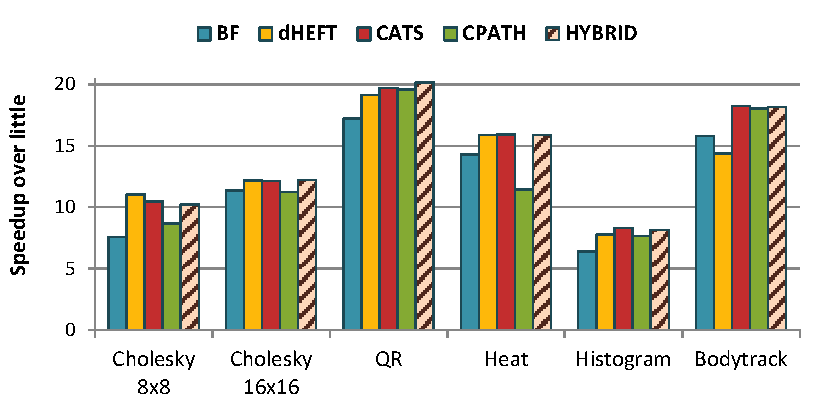
\includegraphics[width=0.7\textwidth]{figures/8cores.pdf}
	\caption{Speedup of CATS, CPATH, HYBRID, dHEFT and BF on 8 cores.}
	\label{BFLinear}
	\vspace{-0.4cm}
\end{figure}
As it is shown in Section~\ref{sec.cats_eval}, the most efficient CATS configuration is when using the simple work stealing and flexible policy (SS FLEX).
The same applies for CPATH and HYBRID schedulers, thus the results presented in this section refer to this configuration of the schedulers. 
Figure~\ref{BFLinear} shows the speedup of CATS, CPATH, HYBRID, dHEFT and BF when running the applications on all eight cores of the Odroid-XU3. Cholesky and Integral Histogram operate on single-precision data, while QR and Heat Diffusion operate on double-precision. 
Double-precision applications get larger speedups over one little core because they benefit from a larger performance ratio when running on a big core. In the case of Bodytrack, the out-of-order processing power of the big cores helps on the efficient execution and creates a high performance ratio between big and little cores. 
For most of the cases, CATS scales better than the rest of the schedulers. 
The shortening of the critical path by running all critical tasks on big cores effectively reduces total execution time when running on all cores. 
CPATH scheduler does not achieve as high speedup as the other heterogeneous scheduling approaches but it still outperforms the baseline (BF) approach.

Figure~\ref{avg_all} shows the average speedup obtained for each scheduler and machine set-up. 
Overall, the heterogeneous schedulers outperform the platform-unaware BF scheduler.
Specifically, CATS and HYBRID achieve a higher speedup by detecting critical tasks.
We observe that their performance is approximately the same and this is due to the fact that HYBRID exploits the same CATS criticality in case the execution time of the task is not yet resolved.
CPATH is less effective due to the additional overheads of the top-to-bottom TDG traversal.
Since the evaluated dHEFT version is improved from previous studies~\cite{Chronaki:ICS2015}, it shows better performance, although it still does not reach the efficiency of CATS and HYBRID because of its task criticality agnosticism.

Moving in more detail, Figure~\ref{speedup} shows the speedup obtained for each application,  scheduler and machine set-up.
We classify the benchmarks according to their task cost variability to easier explain the results.

%------ HEAT ---------- very low variability


Heat diffusion is the kernel with the lowest task variability (e.g. the most homogeneous benchmark) as shown in Figure~\ref{heat_dist}.
CATS, HYBRID and dHEFT increase the performance of heat by 10\% on 8 cores and obtain similar results for the other numbers of cores by rearranging the tasks according to the type of the resources.
Due to its high per-task overheads shown on Table~\ref{tab.sched.apps}
%(CATS: 145.17us per task, CPATH: 748.84us per task, BF: 78.04us per task HYBRID: 170us per task)
 and the homogeneity of the benchmark, CPATH scheduler cannot outperform BF scheduler. 
Moreover, for this benchmark, CPATH detects only 23\% of the tasks to be critical while CATS and HYBRID detect approximately 54\%, when running on 8 cores.
This happens because with CPATH, it is more likely to have zero-priority tasks during the task submission step, due to the post-exit task priority assignment that the algorithm introduces. 
These tasks are considered non-critical, which limits the utilization of the big cores with CPATH. 
%the priorities of the tasks are computed more slowly with CPATH so during task submission there are many tasks with zero priority that are considered non-critical.
%Moreover, as Table~\ref{tab.critical} shows CPATH detects only 23\% of the tasks to be critical while CATS and HYBRID both detect approximately 54\% when running on 8 cores. 
%This limits the utilization of the big cores with CPATH.

%---------- CHOLESKY 16x16 ------------ low variability

Cholesky 16$\times$16 has also low task cost variability. 
The improvements of CATS, dHEFT and HYBRID over BF are limited to around 7\% when running on 8 cores.
These schedulers perform almost the same for the rest numbers of cores and CPATH performs almost the same as BF. 
The increased overheads of CPATH do not pay off with better schedules since, for the same reason as in the case of Heat diffusion, only 10\% of the tasks are marked as critical on 8 cores (while 21\% CATS and 16\% HYBRID).

%--------- BODYTRACK --------------- low variability - very high number of tasks

Bodytrack shows low task cost variability, since 99\% of its tasks have similar execution times.
In this case, contrarily to the previous benchmarks CPATH manages to achieve similar speedups to CATS and HYBRID and outperform BF by up to 15\%.
This is due to the very high number of tasks of bodytrack; CPATH overcomes its overheads by using the detected task execution times for a higher number of tasks.
In other words, the learning phase of CPATH becomes a smaller proportion of the total execution of the benchmark.
Since bodytrack has so many tasks, the per-task overhead of CPATH is around 120us while for CATS it is 93us.
On the other hand, dHEFT shows poor performance because of the overheads of analyzing a TDG with a high number of tasks to compute the earliest finish time schedule.

\begin{figure}[!tr]
	\centering
  	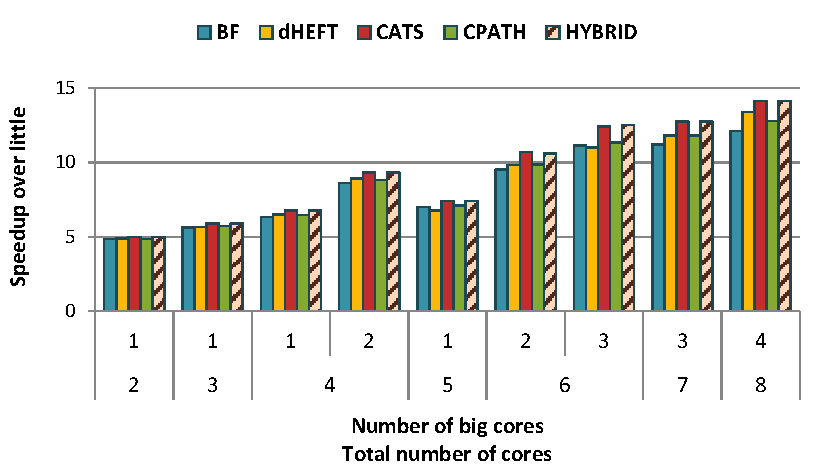
\includegraphics[width=0.7\textwidth]{figures/average_all.pdf}
  	\caption{Average speedups obtained for each scheduler}
  	\label{avg_all}
  	\vspace{-0.5cm}
\end{figure}  

%---------- HISTOGRAM --------------- medium variability - good amount of tasks (2048)

Integral histogram is characterized by medium task cost variability and high amount of tasks.
This benchmark is dependency intensive with limited parallelism, which makes scheduling decisions very important.
CATS and HYBRID schedulers achieve the best results since they focus more on the TDG structure and dependencies, improving BF by 30\% and 27\% respectively.
CPATH and dHEFT are slightly less efficient and improve BF by 19 and 21\% respectively.

%---------- CHOLESKY 8x8 -------------- high variability but very few tasks

For Cholesky 8$\times$8, the heterogeneous schedulers CATS, HYBRID and dHEFT constantly improve the performance of BF and reach up to 45\% improvement on 8 cores.
It is observed here that dHEFT indeed performs better when the number of tasks is limited as this workload has 120 tasks in total.
The additional overheads of CPATH do not compensate with increased performance in this case because there are not enough tasks to apply the better scheduling.

%---------------- QR ------------ the highest variability and good number of tasks (1496)

QR factorization is the highest task cost variability benchmark as shown in Figure~\ref{qr_dist}.
This is the reason why HYBRID gradually outperforms CATS as we increase the number of cores.
With a small additional overhead,
%(CATS: 1419us while HYBRID: 14514us per-task overhead)
as Table~\ref{tab.sched.apps} shows, HYBRID manages to detect critical tasks that reside on the critical path and boost their execution reaching 17\% improvement over the baseline.
For this benchmark, CPATH also reaches a 13\% improvement over BF since task cost matters in this case. 
However, CPATH speedup is still limited compared to HYBRID because of the higher scheduling overheads which in this case is 1.8$\times$ higher than CATS overheads.
dHEFT also improves BF by finding the earliest executor of each task, but the improvement is limited to 11\% which is lower than the other approaches.
\begin{figure*}[!t]
	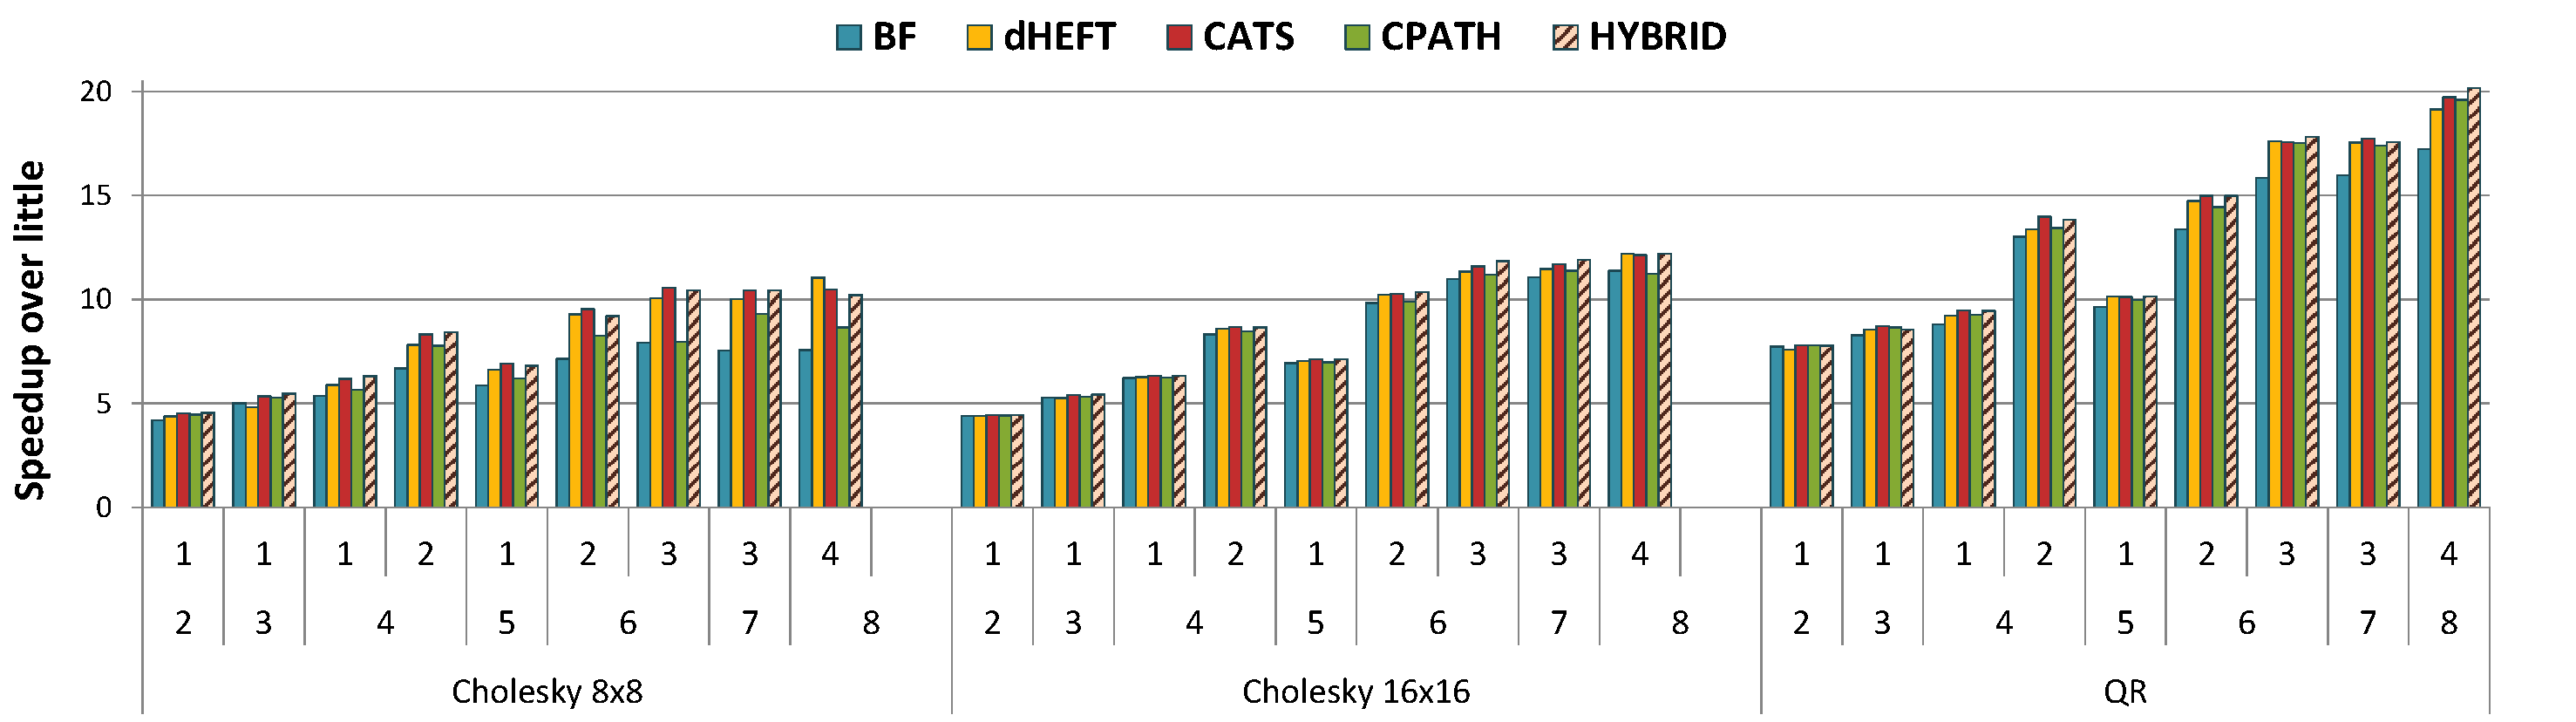
\includegraphics[width=\textwidth]{figures/speedup_apps1.pdf}
	\vspace{-0.4cm}
	
	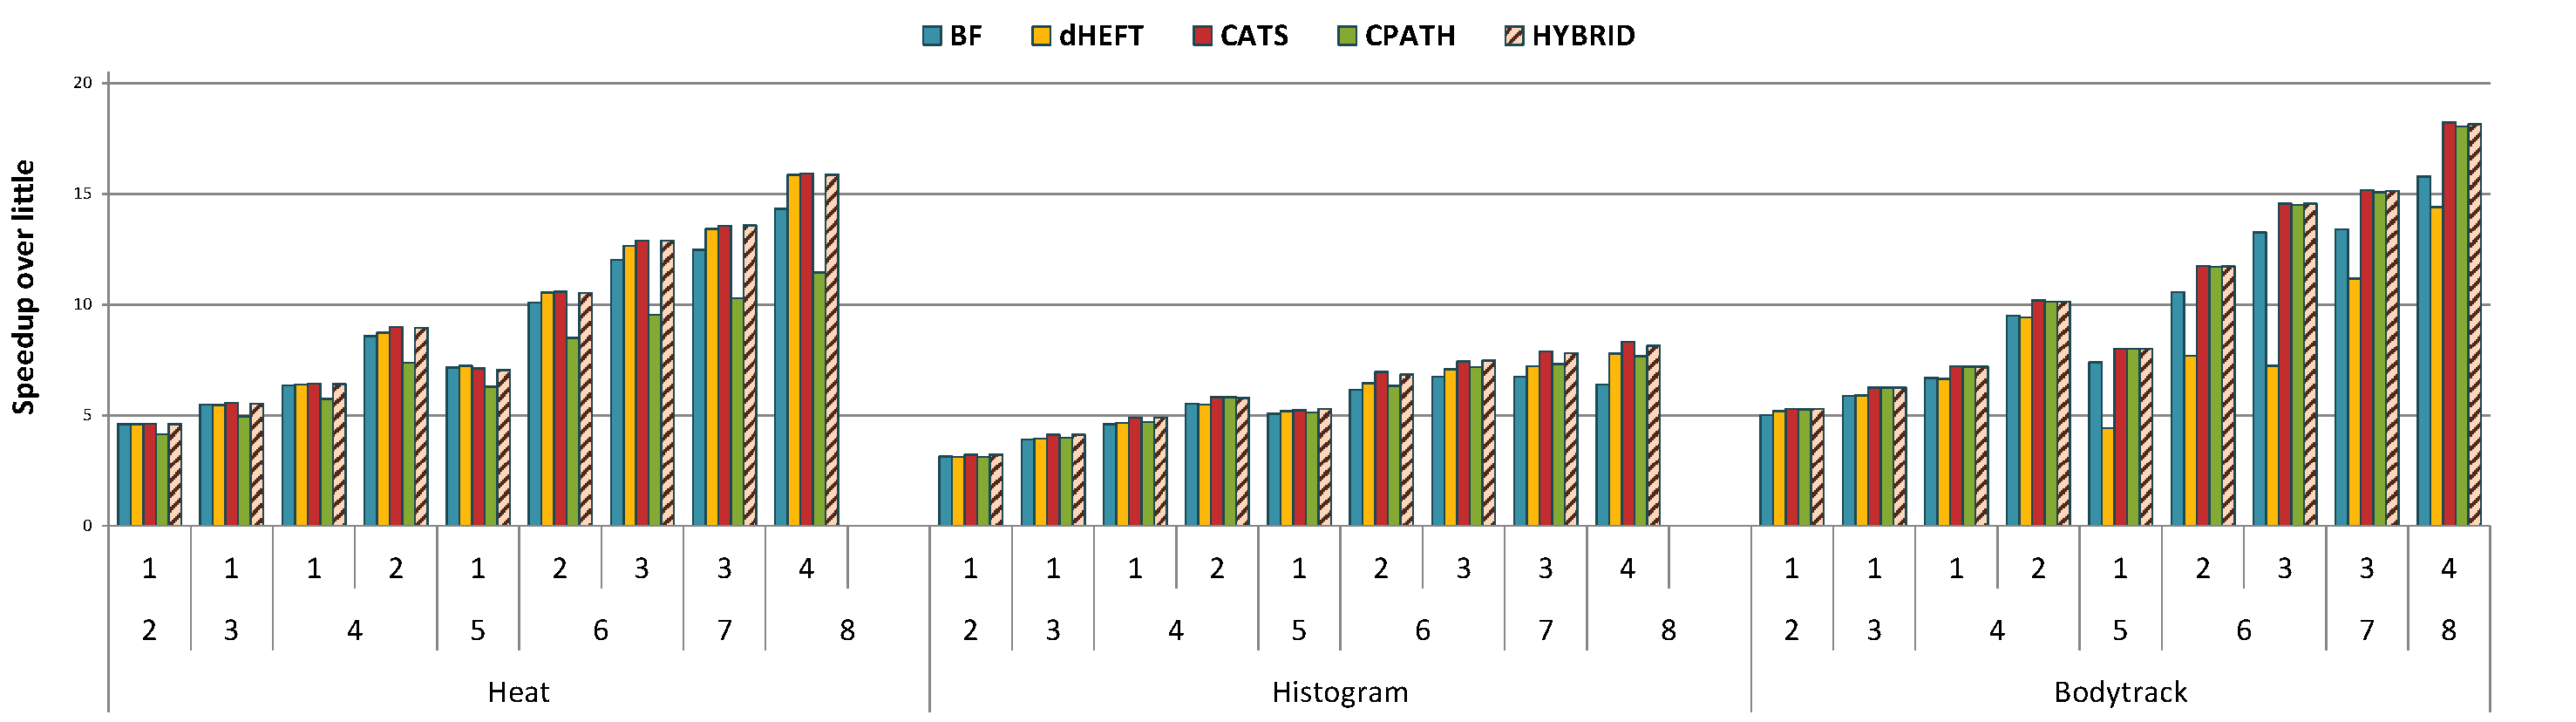
\includegraphics[width=\textwidth]{figures/speedup_apps2.pdf}
	\caption{Speedups obtained for each scheduler and each application}
	\label{speedup}
	\vspace{-0.4cm}
\end{figure*}  

%--------- SUMMARY ---------------

This section showed a straight comparison between different heterogeneous schedulers.
It is important to note that schedulers like CPATH and HYBRID, that detect the time-based critical path, are the best choices when the application has a large amount of tasks.
This is because the additional overheads of these schedulers for critical path computation take place only when there are new tasks on the TDG or when there is a task exit of an untracked tt-is. 
When the TDG has been completely created, and as soon as the cost of every tt-is of the application has been tracked, the schedules of these approaches are purely beneficial.
On the other hand, schedulers like dHEFT perform the same steps for every single task that becomes ready, affecting the entire execution since the exit of a task triggers the execution of its successors that become ready. 
Thus, as the number of tasks is increased, the additional scheduling overheads are increased when using dHEFT-like approaches.
CATS scheduler is an efficient scheduling solution for any number of tasks and task cost distributions.
The additional CATS overheads take place only during task creation and are smaller than CPATH overheads with the drawback of not considering the task execution time.
If we have to choose the best and most generic heterogeneous scheduling approach among the presented schedulers the HYBRID scheduler is the best choice, since it computes an accurate critical path only when it comes at a low cost.


\subsection{Simulations}
To estimate the impact of the heterogeneity-aware schedulers on larger systems, we run three benchmarks using the TaskSim simulator~\cite{AbstrLevels_TACO12}.
The results contain a fixed scheduling overhead for all configurations, regardless of the dynamic overheads during execution (e.g., work stealing).
We simulate Cholesky, QR and Heat diffusion.
These applications feature different levels of task cost variability and have a proper amount of tasks so that the error introduced by the static overhead assumption remains negligible (e.g., bodytrack that creates 408\,525 tasks should not be compared to a 5\,000 task benchmark and static overhead).
For Cholesky, we use an input matrix of 16384$\times$16384 floats creating 512$\times$512 blocks, which results in a 32$\times$32 blocked matrix. This is because the other Cholesky configurations do not scale to 32 cores due to the limited task number. However, the task cost variability is similar to the 16$\times$ 16 input since the task size is not modified. Integral Histogram is excluded from the simulated evaluation because it does not scale beyond 16 cores.

Figures~\ref{cholesky_ts}, \ref{qr_ts} and \ref{heat_ts} show the improvement of dHEFT, CATS, HYBRID and CPATH over BF in systems with 16 and 32 cores for Cholesky, QR and heat respectively. In these experiments, the performance ratio between fast and slow cores is set to 4.5, which is the average performance ratio among the benchmarks. The heterogeneous schedulers utilize fast cores more effectively than BF, which results in larger improvements with higher number of fast cores. 

Figure~\ref{cholesky_ts} shows the improvement of the schedulers over the baseline for Cholesky. The improvement for 16 cores is comparatively small. This is due to the increased problem size used in this experiment.
This benchmark creates a small amount of critical tasks in the 32$\times$32 input, which makes the workload less sensitive to critical tasks and limits the improvement of CATS and HYBRID to a maximum of 17\%, while CPATH and dHEFT outperform BF by up to 10\%. 

%\begin{figure*}[!t]
%\begin{subfigure}[b]{0.33\textwidth}
%  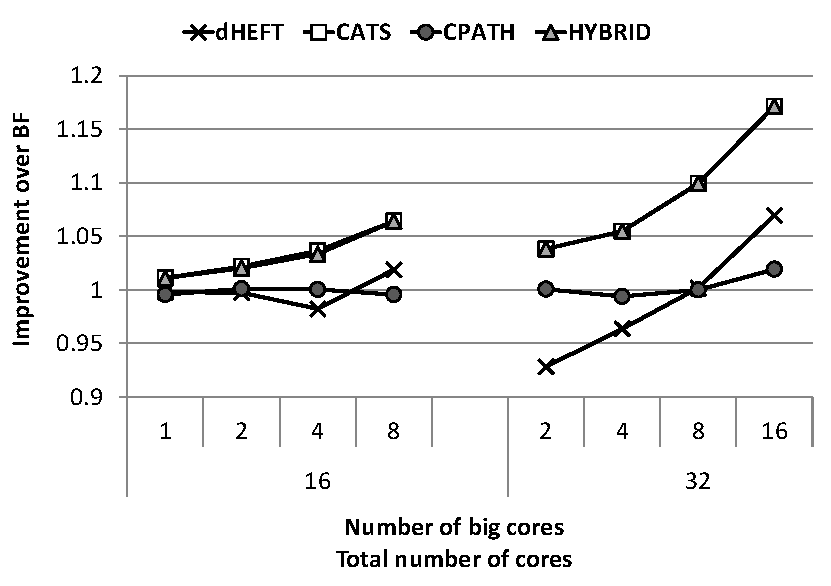
\includegraphics[width=\textwidth]{images/cholesky_TS_tall.pdf}
%  \caption{Cholesky 32$\times$32}
%  \label{cholesky_ts}
%    \vspace{-0.2cm}
%\end{subfigure}
%\begin{subfigure}[b]{0.33\textwidth}
%  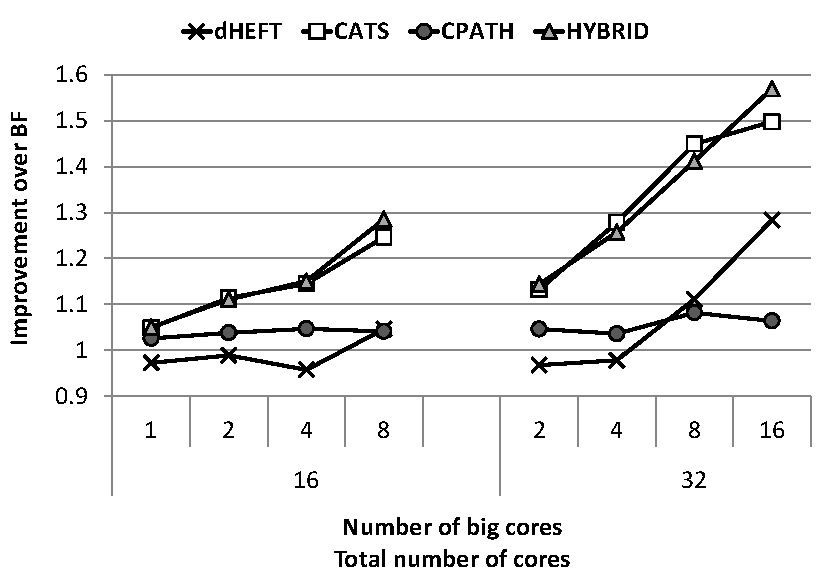
\includegraphics[width=\textwidth]{images/QR_TS_tall.pdf}
%  \caption{QR}
%  \label{qr_ts}
%    \vspace{-0.2cm}
%\end{subfigure}
%\begin{subfigure}[b]{0.33\textwidth}
%  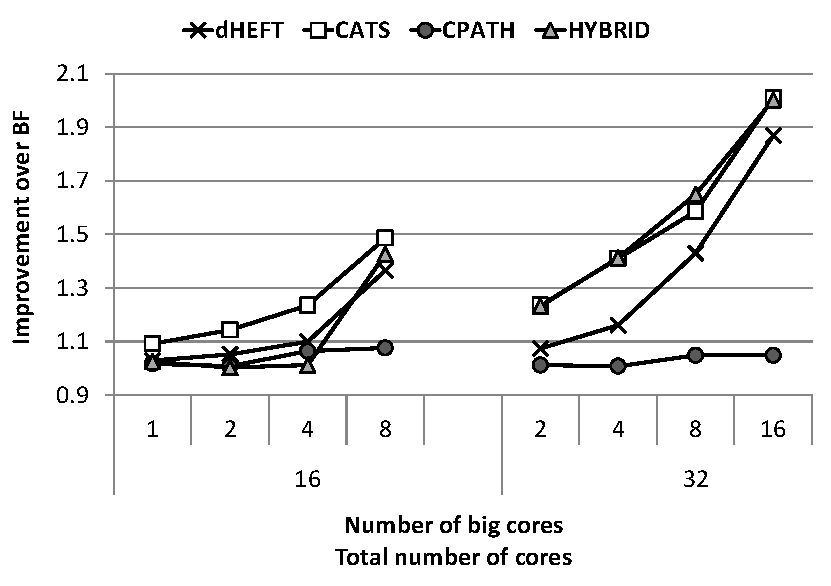
\includegraphics[width=\textwidth]{images/heat_TS_tall.pdf}
%  \caption{Heat diffusion}
%  \label{heat_ts}
%  \vspace{-0.2cm}
%\end{subfigure}  
%\caption{Improvement of heterogeneous schedulers over BF for simulated 16 and 32 core heterogeneous systems}
%\vspace{-0.5cm}
%\end{figure*}

\begin{figure}[!t]
	\centering
	%\subfloat[Cholesky 32$\times$32]{
  		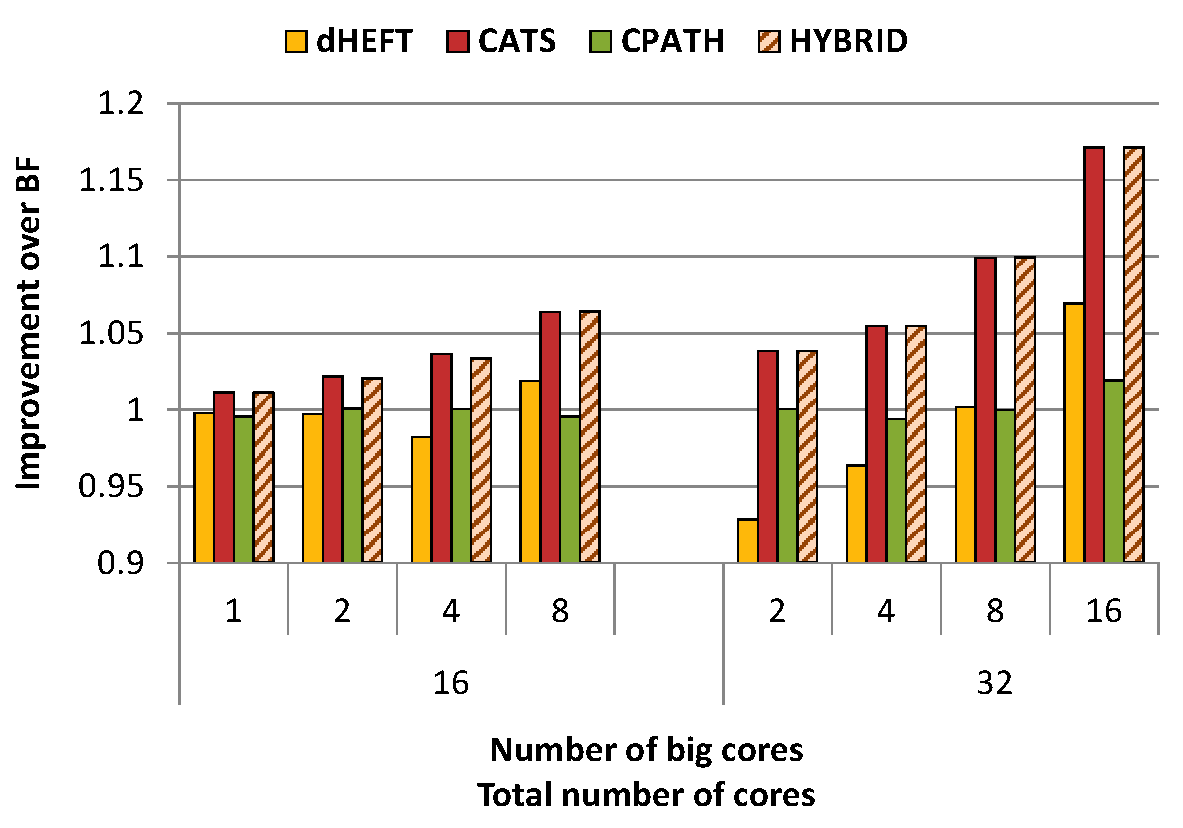
\includegraphics[width=0.65\textwidth]{figures/cholesky_TS_tall.pdf}
		\caption{Improvement of heterogeneous schedulers over BF for simulated 16 and 32 core heterogeneous systems for Cholesky 32$\times$32.}
  		\label{cholesky_ts}
	%}
\end{figure}
%    \vspace{-0.2cm}
%	\subfloat[QR]{
\begin{figure}[h]
	\centering
	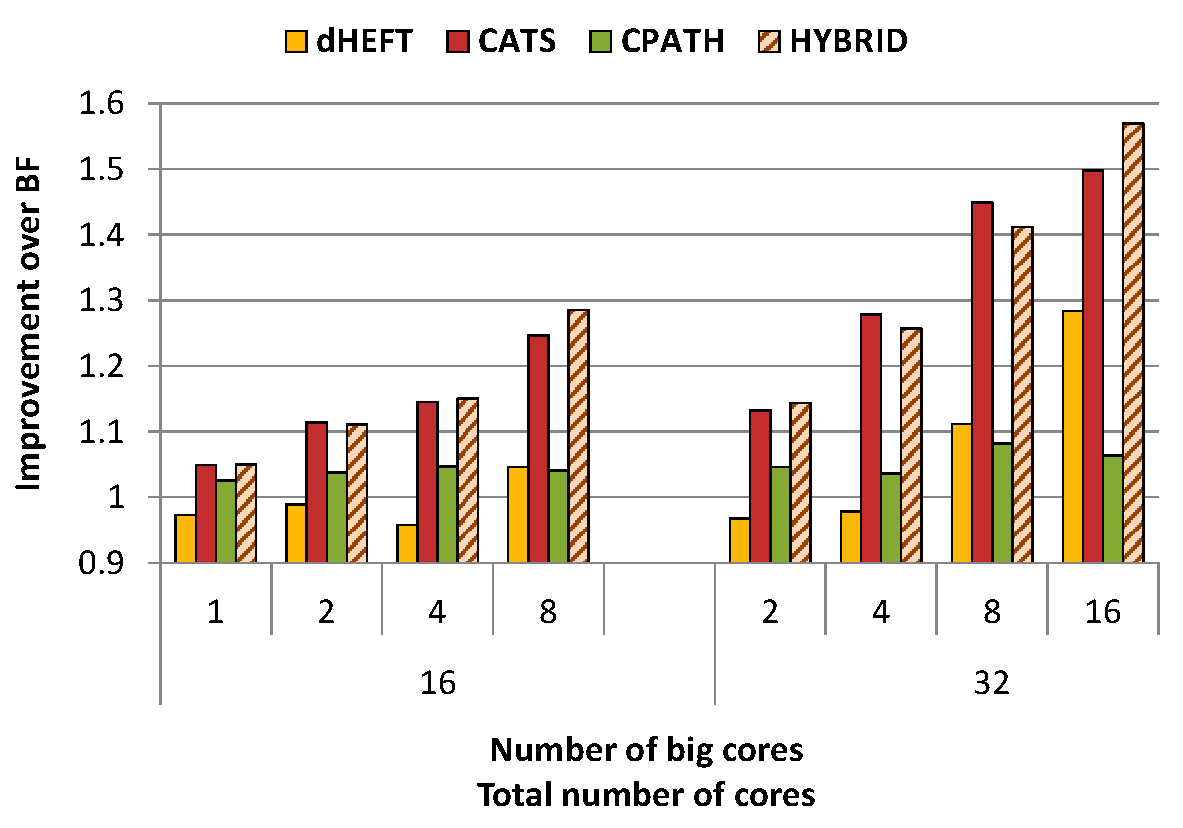
\includegraphics[width=0.65\textwidth]{figures/QR_TS_tall.pdf}
	\caption{Improvement of heterogeneous schedulers over BF for simulated 16 and 32 core heterogeneous systems for QR.}
	\label{qr_ts}
	
\end{figure}
%  	}
%\\
    %\vspace{-0.2cm}
%	\subfloat[Heat diffusion]{
\begin{figure}
	\centering
  		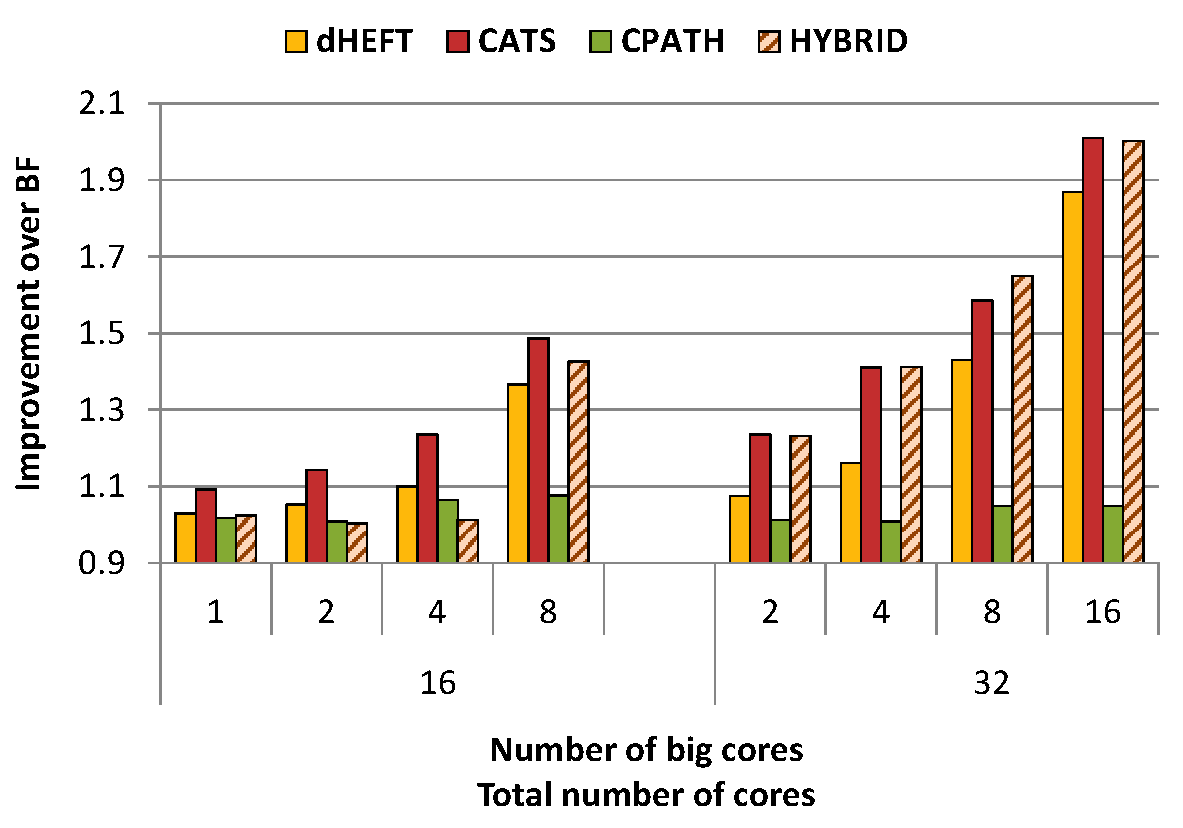
\includegraphics[width=0.65\textwidth]{figures/heat_TS_tall.pdf}
  		\caption{Improvement of heterogeneous schedulers over BF for simulated 16 and 32 core heterogeneous systems for heat diffusion.}
  		\label{heat_ts}
\end{figure}
%  	}
%  \vspace{-0.2cm}
%	\caption{Improvement of heterogeneous schedulers over BF for simulated 16 and 32 core heterogeneous systems}
%\vspace{-0.5cm}
%\end{figure}

Figure~\ref{qr_ts} shows that the best option for QR, the application with the highest task cost variability, on systems with 16 or 32 cores is the HYBRID scheduler, as was also shown in the real platform evaluation, bringing improvements of 30 and 56\%.
CATS also performs well but CPATH falls short in detecting an appropriate amount of critical tasks which makes the little cores overloaded and the big cores waste their resources in work stealing.

For heat diffusion, Figure~\ref{heat_ts} shows that CATS achieves the best results outperforming BF by a factor of 2$\times$. Moreover, HYBRID achieves similar results as it performs similar schedules as CATS. However, CPATH fails to achieve optimal results because it overloads the big cores during the learning phase while the little cores remain under-utilized.


%Depending on the system and according to the application, the optimal solution for this can be found and utilize such systems effectively.
